% Options for packages loaded elsewhere
\PassOptionsToPackage{unicode}{hyperref}
\PassOptionsToPackage{hyphens}{url}
\PassOptionsToPackage{dvipsnames,svgnames,x11names}{xcolor}
%
\documentclass[12pt]{article}
\usepackage{amsmath,amssymb}
\usepackage{iftex}
\ifPDFTeX
  \usepackage[T1]{fontenc}
  \usepackage[utf8]{inputenc}
  \usepackage{textcomp} % provide euro and other symbols
\else % if luatex or xetex
  \usepackage{unicode-math} % this also loads fontspec
  \defaultfontfeatures{Scale=MatchLowercase}
  \defaultfontfeatures[\rmfamily]{Ligatures=TeX,Scale=1}
\fi
\usepackage{lmodern}
\ifPDFTeX\else
  % xetex/luatex font selection
\fi
% Use upquote if available, for straight quotes in verbatim environments
\IfFileExists{upquote.sty}{\usepackage{upquote}}{}
\IfFileExists{microtype.sty}{% use microtype if available
  \usepackage[]{microtype}
  \UseMicrotypeSet[protrusion]{basicmath} % disable protrusion for tt fonts
}{}
\makeatletter
\@ifundefined{KOMAClassName}{% if non-KOMA class
  \IfFileExists{parskip.sty}{%
    \usepackage{parskip}
  }{% else
    \setlength{\parindent}{0pt}
    \setlength{\parskip}{6pt plus 2pt minus 1pt}}
}{% if KOMA class
  \KOMAoptions{parskip=half}}
\makeatother
\usepackage{xcolor}
\usepackage[top=1in,left=1in,right=1in,bottom=1in,heightrounded]{geometry}
\usepackage{longtable,booktabs,array}
\usepackage{calc} % for calculating minipage widths
% Correct order of tables after \paragraph or \subparagraph
\usepackage{etoolbox}
\makeatletter
\patchcmd\longtable{\par}{\if@noskipsec\mbox{}\fi\par}{}{}
\makeatother
% Allow footnotes in longtable head/foot
\IfFileExists{footnotehyper.sty}{\usepackage{footnotehyper}}{\usepackage{footnote}}
\makesavenoteenv{longtable}
\usepackage{graphicx}
\makeatletter
\def\maxwidth{\ifdim\Gin@nat@width>\linewidth\linewidth\else\Gin@nat@width\fi}
\def\maxheight{\ifdim\Gin@nat@height>\textheight\textheight\else\Gin@nat@height\fi}
\makeatother
% Scale images if necessary, so that they will not overflow the page
% margins by default, and it is still possible to overwrite the defaults
% using explicit options in \includegraphics[width, height, ...]{}
\setkeys{Gin}{width=\maxwidth,height=\maxheight,keepaspectratio}
% Set default figure placement to htbp
\makeatletter
\def\fps@figure{htbp}
\makeatother
\setlength{\emergencystretch}{3em} % prevent overfull lines
\providecommand{\tightlist}{%
  \setlength{\itemsep}{0pt}\setlength{\parskip}{0pt}}
\setcounter{secnumdepth}{-\maxdimen} % remove section numbering
% Make \paragraph and \subparagraph free-standing
\makeatletter
\ifx\paragraph\undefined\else
  \let\oldparagraph\paragraph
  \renewcommand{\paragraph}{
    \@ifstar
      \xxxParagraphStar
      \xxxParagraphNoStar
  }
  \newcommand{\xxxParagraphStar}[1]{\oldparagraph*{#1}\mbox{}}
  \newcommand{\xxxParagraphNoStar}[1]{\oldparagraph{#1}\mbox{}}
\fi
\ifx\subparagraph\undefined\else
  \let\oldsubparagraph\subparagraph
  \renewcommand{\subparagraph}{
    \@ifstar
      \xxxSubParagraphStar
      \xxxSubParagraphNoStar
  }
  \newcommand{\xxxSubParagraphStar}[1]{\oldsubparagraph*{#1}\mbox{}}
  \newcommand{\xxxSubParagraphNoStar}[1]{\oldsubparagraph{#1}\mbox{}}
\fi
\makeatother
% definitions for citeproc citations
\NewDocumentCommand\citeproctext{}{}
\NewDocumentCommand\citeproc{mm}{%
  \begingroup\def\citeproctext{#2}\cite{#1}\endgroup}
\makeatletter
 % allow citations to break across lines
 \let\@cite@ofmt\@firstofone
 % avoid brackets around text for \cite:
 \def\@biblabel#1{}
 \def\@cite#1#2{{#1\if@tempswa , #2\fi}}
\makeatother
\newlength{\cslhangindent}
\setlength{\cslhangindent}{1.5em}
\newlength{\csllabelwidth}
\setlength{\csllabelwidth}{3em}
\newenvironment{CSLReferences}[2] % #1 hanging-indent, #2 entry-spacing
 {\begin{list}{}{%
  \setlength{\itemindent}{0pt}
  \setlength{\leftmargin}{0pt}
  \setlength{\parsep}{0pt}
  % turn on hanging indent if param 1 is 1
  \ifodd #1
   \setlength{\leftmargin}{\cslhangindent}
   \setlength{\itemindent}{-1\cslhangindent}
  \fi
  % set entry spacing
  \setlength{\itemsep}{#2\baselineskip}}}
 {\end{list}}
\usepackage{calc}
\newcommand{\CSLBlock}[1]{\hfill\break\parbox[t]{\linewidth}{\strut\ignorespaces#1\strut}}
\newcommand{\CSLLeftMargin}[1]{\parbox[t]{\csllabelwidth}{\strut#1\strut}}
\newcommand{\CSLRightInline}[1]{\parbox[t]{\linewidth - \csllabelwidth}{\strut#1\strut}}
\newcommand{\CSLIndent}[1]{\hspace{\cslhangindent}#1}
\usepackage{booktabs}
\usepackage{caption}
\usepackage{longtable}
\usepackage{colortbl}
\usepackage{array}
\makeatletter
\@ifpackageloaded{caption}{}{\usepackage{caption}}
\AtBeginDocument{%
\ifdefined\contentsname
  \renewcommand*\contentsname{Table of contents}
\else
  \newcommand\contentsname{Table of contents}
\fi
\ifdefined\listfigurename
  \renewcommand*\listfigurename{List of Figures}
\else
  \newcommand\listfigurename{List of Figures}
\fi
\ifdefined\listtablename
  \renewcommand*\listtablename{List of Tables}
\else
  \newcommand\listtablename{List of Tables}
\fi
\ifdefined\figurename
  \renewcommand*\figurename{Figure}
\else
  \newcommand\figurename{Figure}
\fi
\ifdefined\tablename
  \renewcommand*\tablename{Table}
\else
  \newcommand\tablename{Table}
\fi
}
\@ifpackageloaded{float}{}{\usepackage{float}}
\floatstyle{ruled}
\@ifundefined{c@chapter}{\newfloat{codelisting}{h}{lop}}{\newfloat{codelisting}{h}{lop}[chapter]}
\floatname{codelisting}{Listing}
\newcommand*\listoflistings{\listof{codelisting}{List of Listings}}
\makeatother
\makeatletter
\makeatother
\makeatletter
\@ifpackageloaded{caption}{}{\usepackage{caption}}
\@ifpackageloaded{subcaption}{}{\usepackage{subcaption}}
\makeatother
\makeatletter
\@ifpackageloaded{sidenotes}{}{\usepackage{sidenotes}}
\@ifpackageloaded{marginnote}{}{\usepackage{marginnote}}
\makeatother
\ifLuaTeX
  \usepackage{selnolig}  % disable illegal ligatures
\fi
\usepackage{bookmark}
\IfFileExists{xurl.sty}{\usepackage{xurl}}{} % add URL line breaks if available
\urlstyle{same}
\hypersetup{
  pdftitle={Community Water System Service Areas},
  pdfauthor={Andrew Murray \& Alex Hall},
  colorlinks=true,
  linkcolor={blue},
  filecolor={Maroon},
  citecolor={blue},
  urlcolor={blue},
  pdfcreator={LaTeX via pandoc}}

\title{Community Water System Service Areas}
\usepackage{etoolbox}
\makeatletter
\providecommand{\subtitle}[1]{% add subtitle to \maketitle
  \apptocmd{\@title}{\par {\large #1 \par}}{}{}
}
\makeatother
\subtitle{Documentation}
\author{Andrew Murray \& Alex Hall}
\date{}


%% ADD EPA SPECIFIC FUNCTIONS HERE

%% Hold all figure positions
\usepackage{float}
\floatplacement{figure}{H}

% TODO: Add custom LaTeX header directives here
\usepackage{fontspec}
\setmainfont{Calibri}

%% Create title page
\usepackage{xcolor}
\usepackage{graphicx}
\usepackage{tikz}
\usepackage[absolute]{textpos}

% text box setup
\setlength{\TPHorizModule}{0.25in}
\setlength{\TPVertModule}{\TPHorizModule}
\textblockorigin{0in}{0in}

%% Define Colors
\definecolor{epagreen}{HTML}{00673E}

%% funtion to insert blank pages
\usepackage{afterpage}

\newcommand\blankpage{%
    \null
    \thispagestyle{empty}%
    \addtocounter{page}{-1}%
    \newpage}

%% Headers
\usepackage{fancyhdr}
\pagestyle{fancy}
\fancyhead{} % clear all header fields
\fancyhead[RO,LE]{EPA 600/XXX/XXX | May 2024 | www.epa.gov/research}

\begin{document}

%% COVER PAGE
\thispagestyle{empty}
\pagecolor{epagreen}
% EPA Logo
\begin{tikzpicture}[remember picture,overlay,shift={(current page.north west)}]
\node[anchor=north west,xshift=0.93in,yshift=-0.43in]{\includegraphics[width=2in]{_extensions/ORD_ceser_pdf/img/epa_logo_vert_white.png}};
\end{tikzpicture}
  
% Report Number
\begin{textblock}{16}(18,2)
\small\textcolor{white}{EPA 600/XXX/XXX | May 2024 | www.epa.gov/research}
\end{textblock}
  
% Title
\begin{textblock}{28}(4,10)
\huge\textcolor{white}{Community Water System Service Areas}
\end{textblock}
  
% Subtitle
\begin{textblock}{28}(4,12)
\textcolor{white}{Documentation}
\end{textblock}

% Cover Image
\begin{tikzpicture}[remember picture,overlay,shift={(current page.north west)}]
\node[anchor=north west,xshift=-0.05in,yshift=-3.6in]{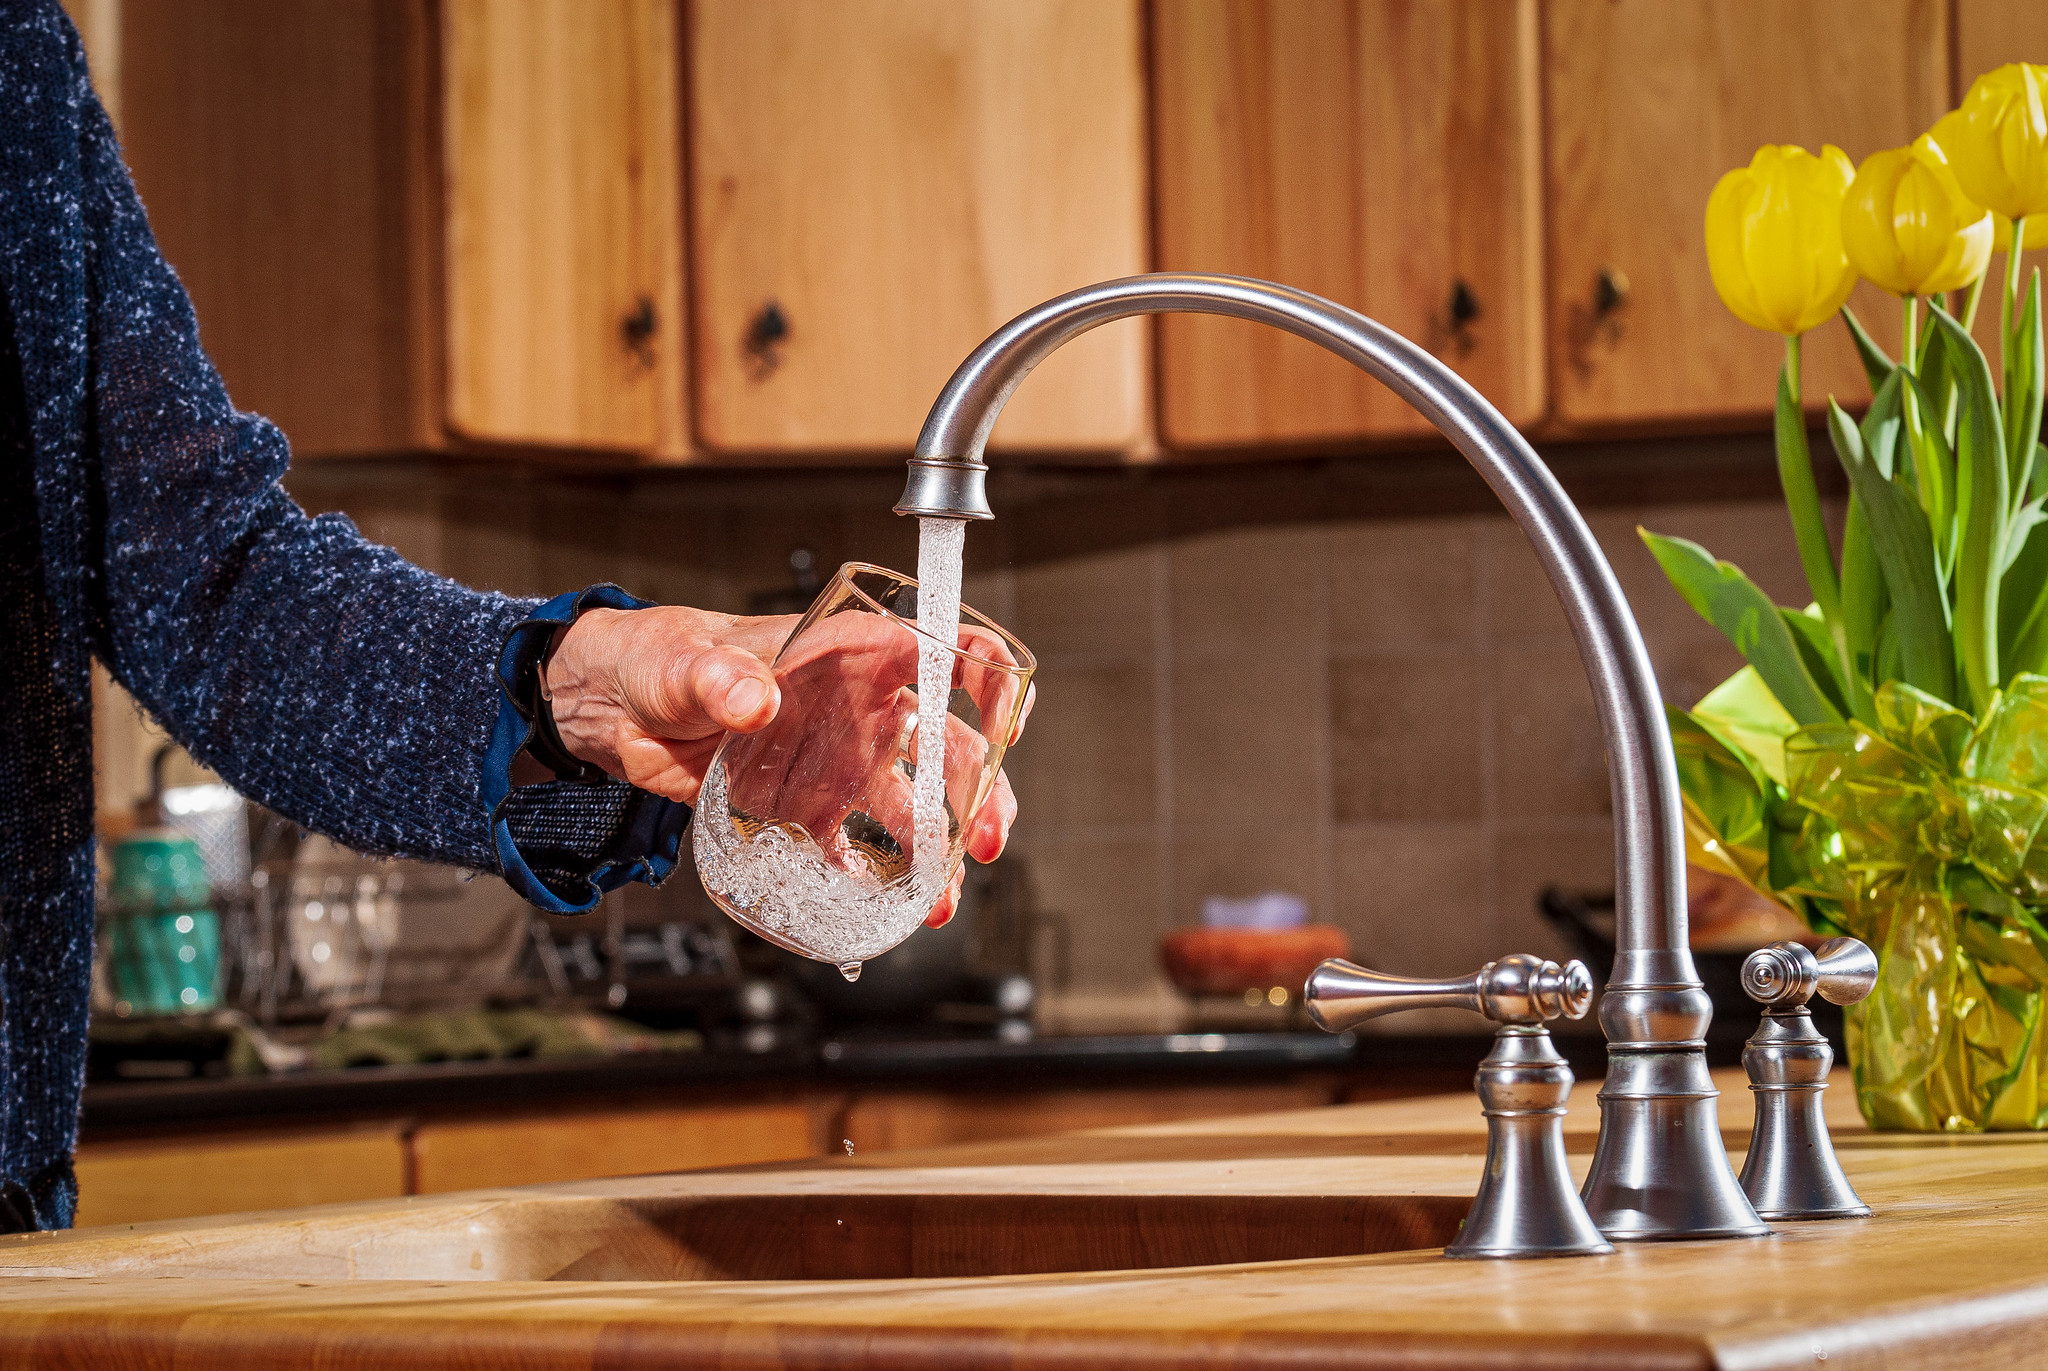
\includegraphics[width=\paperwidth]{img/EPA_Water.jpg}};
\end{tikzpicture}

% Organization
\begin{textblock}{28}(4,39)
\small\textcolor{white}{Office of Research and Development\newline Center for Environmental Solutions and Emergency Response}
\end{textblock}


%% Blank Page
\clearpage
\pagecolor{white}
\thispagestyle{empty}
\hfill
\clearpage

%% Title Page
% \pagestyle{plain}
\setcounter{page}{1}
\pagenumbering{roman}
\begin{center}

\begin{huge}
\textcolor{black}{Community Water System Service Areas}\\
\end{huge}

\normalsize Documentation

\vspace{1in}
by
\\Andrew Murray \& Alex Hall
\\Center for Environmental Solutions and Emergency Response
\\Cincinnati, OH 45268
\end{center}
\clearpage


%% Disclaimer
\begin{center}
\huge Disclaimers\\
\end{center}

\normalsize

This document is distributed solely for the purpose of pre-dissemination
peer review under applicable information quality guidelines. It has not
been formally disseminated by the U.S. Environmental Protection Agency.
It does not represent and should not be construed to represent any
agency determination or policy.

\clearpage


% 
%% Table of Contents
\renewcommand*\contentsname{Table of contents}
% % {
\hypersetup{linkcolor=blue}
\setcounter{tocdepth}{3}
\tableofcontents
%}
\listoffigures
\listoftables

%% Table of Abbreviations
\clearpage

\Large\bfseries{List of Abbreviations}

\normalsize\mdseries

\begin{table}[ht]
\centering
\begin{tabular}{ll}
  \hline
 Abbreviation & Description \\ 
  \hline
CWS & Community Water System \\ 
  HBSL & Health-Based Screening Level \\ 
  HIFLD & Homeland Infrastructure Foundation-Level Data \\ 
  MCL & Maximum Contaminant Level \\ 
  NHGIS & National Historical Geographic Information System \\ 
  OOB & Out-of-Bag \\ 
  ORD & EPA Office of Research and Development \\ 
  OSM & Open Street Map \\ 
  PWSID & Public Water System Identifier \\ 
  SAB & Service Area Boundary \\ 
  SDWA & Safe Drinking Water Act \\ 
  SDWIS & Safe Drinking Water Information System \\ 
   \hline
\end{tabular}
\end{table}
\clearpage


\pagenumbering{arabic}
\section{Executive Summary}\label{executive-summary}

The Office of Research and Development has released a publicly available
dataset of community water system (CWS) service area boundaries (SAB).
CWS are defined as systems that provide water for human consumption
through pipes or other constructed conveyances to at least 15 service
connections or serves an average of at least 25 people year-round
(\citeproc{ref-cws}{U. EPA 2022}) and represent the source of roughly
84\% of household drinking water in the United States
(\citeproc{ref-murray2021methods}{Murray et al. 2021}). Under the safe
drinking water act (SDWA) and various drinking water rules public water
systems must test and report on the quality of their drinking water
(\citeproc{ref-act1974safe}{Act 1974}).

While water quality has been a top priority for decades, it remains
challenging to determine where households in the United States obtain
their drinking water from. There are over 47,000 active community water
systems in the United States. Knowing the service areas of these
utilities is critical to understanding who is drinking water from where
and will enable a link between Safe Drinking Water Act (SDWA) reporting
and the populations consuming water from specific utilities.

One study, which sampled 931 public supply wells found that ``one or
more chemical contaminants were detected at concentrations greater than
maximum contaminant levels (MCL) or health-based screening levels (HBSL)
in more than one in five (22 percent)'' of sampled wells
(\citeproc{ref-toccalino2010quality}{Toccalino, Norman, and Hitt 2010}).
This substantiates the need for federal requirements; these samples were
collected prior to treatment. Treatment processes, or dilution can
substantially reduce the risk of contaminants getting to the consumer.
While federal standards help reduce the likelihood of contaminated
drinking water, of the total universe of public water systems in the
United States, 6\% reported to have violated a health-based drinking
water standard and 29\% failed to meet at least one monitoring or
reporting requirement in 2022 (\citeproc{ref-epaCompliance}{U. S. EPA
2023}).

Community water systems have testing and reporting requirements that may
increase based on the size of the system, compliance history and local
or state specific requirements. While the source of water for a home may
be a primary determinate of its quality, the type of system (private
well, small or large community water system) can play an equally
important role in the ability for a system to have adequate treatment
processes. Private wells, for example, are not regulated by federal law
and thus the responsibility for testing and treatment generally falls to
the homeowner. It is therefore critical that we understand where people
are sourcing their water, who is consuming the water, and how it is
delivered to their home in order to more completely understand regional
and national trends of water quality and the health impacts to the
public.

Using a combination of public data sources, spatial analysis, and
machine learning, the Office of Research and Development has developed a
national dataset of community water system service areas. Where
available, we collect and include publicly available service areas from
states. Where service areas are not published, we apply two models to
estimate service areas. The first model uses a decision tree method
witch uses data from the 1990 and 2020 Census, community water system
infrastructure data from SDWIS and land cover data to determine, for
each census block, if it is likely to be served by a public water system
or by private sources such as domestic wells.

The second model uses a random forest model, with several additional
variables to determine, for blocks estimated to be served by public
water, the most likely utility to be providing that water. The universe
of community water systems is considered current as of 2023 (Quarter 4).
Out of a total of 47,538 systems, our dataset includes service areas for
44,415 (93.4\%), which represents 99.4\% of the total population served
by community water systems. At present, this dataset does not include
service areas for Puerto Rico or U.S. territories. The data is available
from the
\href{https://epa.maps.arcgis.com/apps/webappviewer/index.html?id=5a9963ca7a594fbd9b0df40050ed704e}{EPA
Community Water System Service Area Viewer}

\subsection{SDWIS Reporting Universe}\label{sdwis-reporting-universe}

The current ORD dataset (Version 1.0), uses the 2023 (Q4) release of
SDWIS data. As of this release, there were a total of 49,396 active
community water systems, which primarily serve residential areas
(Figure~\ref{fig-systemType}). There are many systems, however, which
primarily wholesale water to other systems, meaning they do not directly
serve water to consumers and therefore do not have a service area
boundary. These systems simply source water and deliver it to other
systems, who then serve individual customers. The universe of systems in
our efforts is limited to currently active community water systems which
serve at least 15 service connections or serves an average of at least
25 people for at least 60 days a year. The total number of systems that
fit this criteria for 2023 (Q4) is: 47,538. Currently, this dataset does
not include service areas for U.S. territories (Puerto Rico, American
Samoa, Guam, Commonwealth of the Northern Mariana Islands, U.S. Virgin
Islands).

Community water systems each fall under a primacy agency
(Figure~\ref{fig-statePlot}), which is the agency with primary
responsibility for implementing SDWA, this is typically the state or
territory. The exceptions, where EPA is the primacy agency are Wyoming,
the District of Columbia, and federally recognized tribes excluding
Navajo Nation. Navajo Nation is currently the only tribe with primacy
agency status to enforce SDWA.

\begin{figure}

\centering{

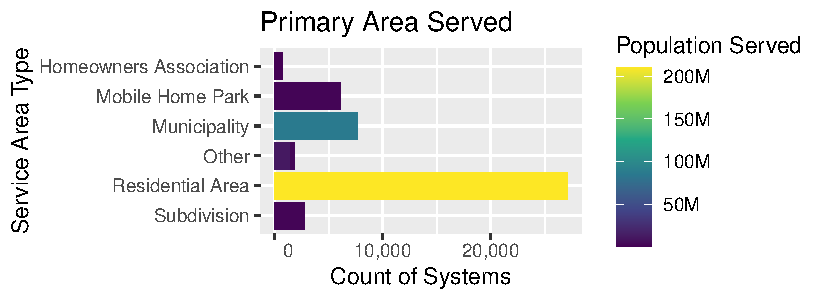
\includegraphics{Documentation_files/figure-pdf/fig-systemType-1.pdf}

}

\caption{\label{fig-systemType}Types of Active Systems in SDWA
Reporting}

\end{figure}%

\begin{figure}

\centering{

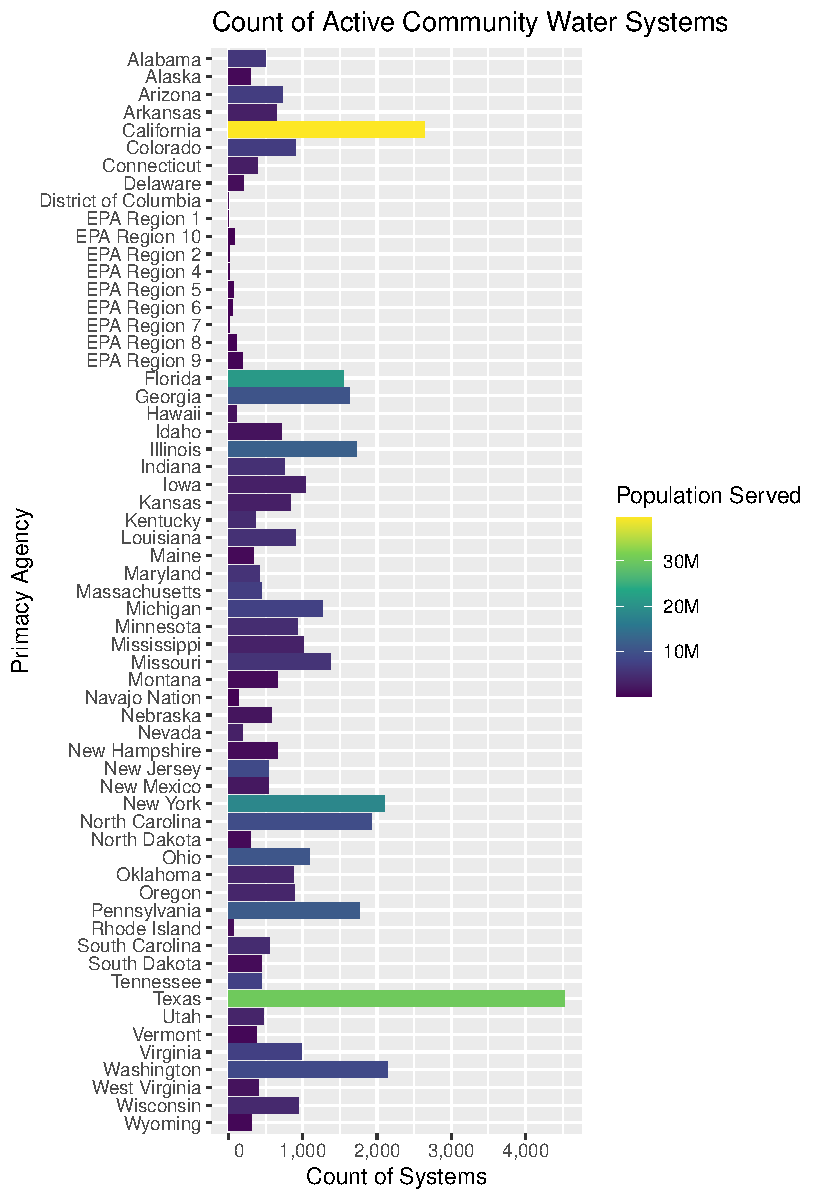
\includegraphics{Documentation_files/figure-pdf/fig-statePlot-1.pdf}

}

\caption{\label{fig-statePlot}Bar plot showing the count of active
community water systems by state, region or territory.}

\end{figure}%

\section{State Data}\label{state-data}

When detailed (accurately drawn and not simplified polygons such as
county or city boundaries) public water service area boundaries are
publicly available from state or municipal sources, we consider those to
be authoritative and use them instead of modeled boundaries. A detailed
review was conducted of available data and used to determine what would
be included in the ORD national dataset versus what would be modeled
(Table~\ref{tbl-stateCounts}). Detailed descriptions of state data are
available in the supplementary materials.

\begin{table}

\caption{\label{tbl-stateCounts}Number of system boundaries from state
and municipal sources included in the ORD dataset. The total number of
systems included is 18,374.}

\begin{minipage}{\linewidth}

\begin{longtable*}{l>{\centering\arraybackslash}p{100px}l>{\centering\arraybackslash}p{100px}l>{\centering\arraybackslash}p{100px}}
\toprule
State & Count of Systems & State & Count of Systems & State & Count of Systems \\ 
\midrule\addlinespace[2.5pt]
AL &     2 & KS &   781 & NY &   308 \\ 
AR &   670 & KY &   367 & OH &     1 \\ 
AZ &   707 & LA &     1 & PA & 1,771 \\ 
CA & 2,814 & MA &     2 & RI &    31 \\ 
CO &     3 & MI &     2 & SC &     2 \\ 
CT &   448 & MS &   361 & TN &   432 \\ 
DC &     1 & MT &     1 & TX & 4,538 \\ 
FL &   420 & NC &   482 & UT &   485 \\ 
GA &     3 & NH &   658 & WA & 1,747 \\ 
IA &     2 & NJ &   560 & WI &     2 \\ 
ID &     2 & NM &   532 & WV &   235 \\ 
IN &     2 & NV &     1 &  &  \\ 
\bottomrule
\end{longtable*}

\end{minipage}%

\end{table}%

\section{Place Matched Service Area
Boundaries}\label{place-matched-service-area-boundaries}

\subsection{Mobile Homes - OSM}\label{mobile-homes---osm}

Mobile home parks may represent community water systems that are smaller
than a census block, which is the base resolution for the models we
create. Therefore, an effort was made to find polygons that represent
specific mobile home parks and tie them to their respective community
water systems. Areas tagged by Open Street Map (OSM) as
`residential=trailer\_park', `residential=mobile', or
`residential=mobile\_home\_park' were extracted from Open Street Map and
fuzzy name matched with community water system names reported to SDWIS.
To find open street map delineated areas, the point locations for mobile
home parks from Homeland Infrastructure Foundation-Level Data (HIFLD)
(\citeproc{ref-hifld}{HIFLD 2023}) was intersected with areas tagged as
`residental=trailer\_park' in open street map. If an intersection
occured, the given names of that mobile home park (from both sources)
were matched with SDWIS reported names.

\subsection{Mobile Homes - Parcels}\label{mobile-homes---parcels}

Where open street map delineated areas were not present, we point
locations of mobile home parks were extracted from HIFLD
(\citeproc{ref-hifld}{2023}). Points were then intersected with polygon
data representing parcels, which were obtained from REGRID
(\citeproc{ref-regrid}{2023}). The name of the mobile home park was then
fuzzy matched with SDWIS reported system names.

\section{Modeled Service Area
Boundaries}\label{modeled-service-area-boundaries}

\subsection{Binary Water Use Model}\label{binary-water-use-model}

A decision tree model was created to determine the probability that a
census block is served by a public water system. This model was levered
in two different ways: 1.) to aid in the 1:1 matching discussed later
and 2.) as a model input (explanatory variable) for the random forest
model. The variables included are listed in Table~\ref{tbl-dtvars}.

\begin{longtable}{l>{\raggedright\arraybackslash}p{300px}}

\caption{\label{tbl-dtvars}Variables included in decision tree model.}

\tabularnewline

\toprule
Variable & Description \\ 
\midrule\addlinespace[2.5pt]
Imperviousness & Urban Imperviousness in percent, derived from the National Land Cover Dataset \\ 
2020 Housing Unit Density & Housing units per square kilometer \\ 
Area & Area in square kilometers \\ 
\% Public Use in 1990 & \% of housing units that reported public water use from 1990 Census \\ 
\% Sewer Use in 1990 & \% of housing units that reported public sewer use from 1990 Census \\ 
1990 Housing Units & Count of housing units in block from 1990 Census \\ 
\% Housing Unit Change 1990-2020 & \% change in housing units between 1990 and 2020 Census \\ 
Distance to Public Water Intake & Distance in kilometers between block centroid and closest public water intake as derived from the Safe Drinking Water Information System \\ 
\bottomrule

\end{longtable}

For census data obtained from the 1990 decennial census, we applied a
spatial weighting technique to estimate the number housing units using
public water for 1990 census blocks based on published data for census
block groups. Census blocks within each block group were ranked from
highest housing unit density to lowest housing unit density. The total
number of housing units using public water systems was known at the
block group level, and this number is then distributed into the most
dense census block first, then the next most dense block and so on until
no more housing units on public water remain. The remainder of housing
units within the less dense blocks are then assumed to be using well
water. This method is used because of the statistical relationship that
exists between housing unit density and public water use: we know that
the densest areas are most likely to be served by public water. To
validate the model, public water systems from three states (New Jersey,
Connecticut \& California) were joined to census blocks to classify the
intersecting blocks as public water users. These three states were
chosen based on the completeness and detail of their service area
boundaries. The final decision tree model (Figure~\ref{fig-dt})
predicted the type of water supply correctly in 93.14\% of blocks in the
testing dataset which was removed prior to training. The accuracy of
public use (sensitivity) was 95\% and the accuracy of private use
(specificity) was 81\%. A secondary validation was performed using data
from Washington, which was never exposed to the model for training
(Table~\ref{tbl-wash}). We determined the Washington data to be robust
and thus it served as both a validation of the model and provided
confidence that the model could be applied in states where the model was
not trained. For more details on this initial model, refer to the
\href{https://github.com/USEPA/ORD_Water_Source_2020}{2020 Water Source
Model GitHub Site}.

\begin{table}

\caption{\label{tbl-wash}Confusion matrix showing both decision tree
predictions~for both the out of bag testing set and data from
Washington.}

\centering{

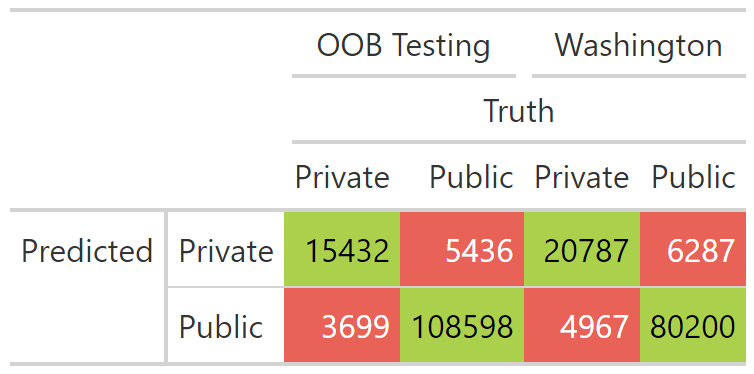
\includegraphics[width=3in,height=\textheight]{img/performance_tbl.png}

}

\end{table}%

\begin{figure}

\centering{

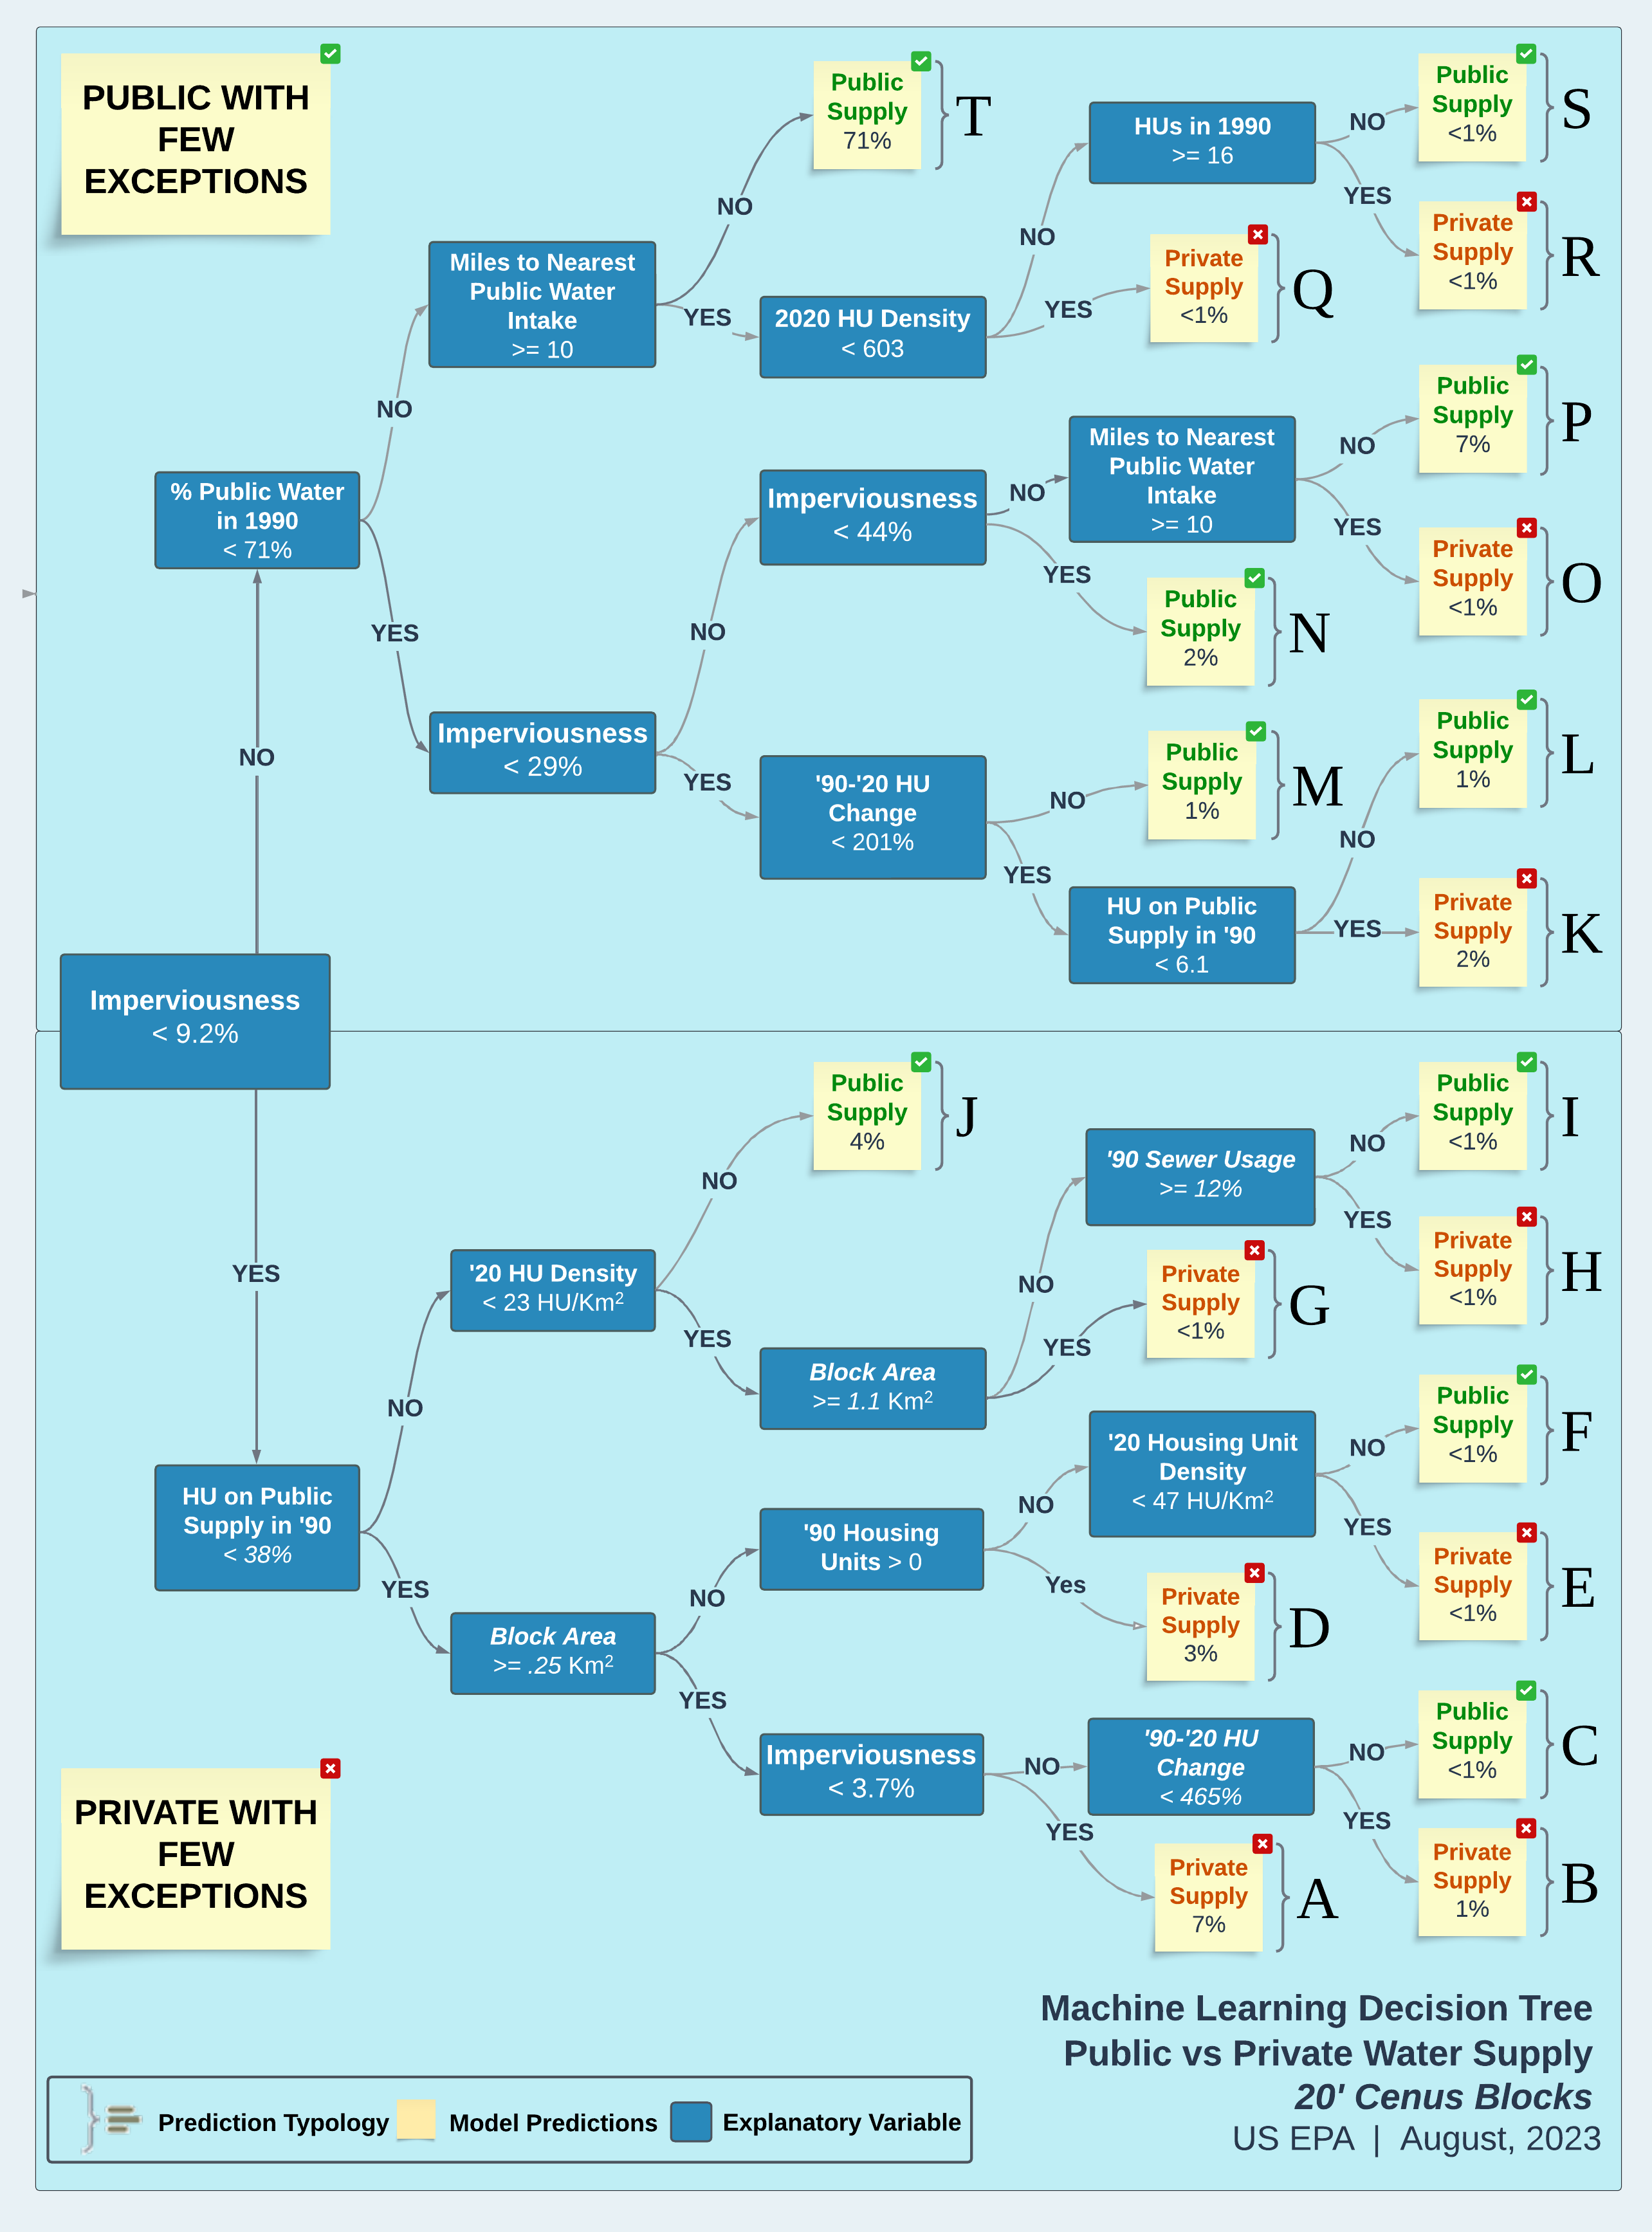
\includegraphics{img/DT.png}

}

\caption{\label{fig-dt}Visualization of decision tree to predict whether
a census block is served by a public water system.}

\end{figure}%

\subsection{1:1 Match}\label{match}

Census blocks that are predicted to be served by public water by the
binary water use model (Figure~\ref{fig-dt}) are `aggregated' or
`dissolved' spatially, meaning they are combined with any contiguous
blocks that are also estimated to be served by public water systems into
larger polygons. A public probability threshold of .7 and higher was
used to classify block as exclusively on public water. These aggregated
polygons are then spatially joined with facility locations from SDWIS,
which include intakes, wells, and treatment plants. If a single
aggregated area can only be associated with facilities from a single
public water system, that area is assigned its associated PWSID.

As a general approach to modeling, simplicity is typically preferred
over complexity. The 1:1 matching was an attempt to resolve system
assignments in a very simple way, eliminating the need for more complex
random forest modeling. Approximately 8,000 (\textasciitilde17\%)
systems were assigned (or matched) using this method. This method
leveraged the decision tree output to determine system boundary size.
Since the model provided confidence levels associated to every block,
from 0=confident that that the block is privately supplied; to 1=
confident that block is publicly supplied. We found that a value of 0.7
closely approximated the system boundary size and shape when compared to
state supplied boundaries. After applying this criteria, we sought to
match the system boundaries to their associated PWSID. Spatially
continuous blocks were aggregated together into larger polygons.

To determine a match, we used SDWIS locations (wells, treatment plant,
intakes) and SDWIS locations (reported system addresses that we
geocoded) to conduct a spatial join to the aggregated decision tree
boundaries (at 0.7 confidence). The logic here is that for some systems
there is only one PWS that serves the polygon area---as opposed to a
more complex nested set of systems within a single polygon. More complex
systems are mainly associated with urban and suburban areas where the
simple systems are largely associated with smaller to mid-size towns in
rural areas. The other assumption we had was that it is more likely that
a system's infrastructure is close to the population that it serves than
farther away.

We performed a spatial join on all decision tree boundaries and SDWIS
locations. If more than one unique system was joined, those boundaries
were returned for random forest modeling. If only one PWSID was returned
for a polygon we validated that the joins were associated with the
correct PWS. To do this we performed a graphical validation method by
regressing the service connection of the joined public water system
against the sum 2020 housing units within the modeled boundary. Because
each state uses a different formula for calculating the service
connections, these regressions had to be limited to intra-state
comparisons. In other words, the regressions coefficients could vary
widely between states, creating an ``apples-to-oranges'' comparison. The
regression was trimmed to systems that fell close to the 1-to-1
regression line. Systems that deviated from that line were removed for
later random forest matching. Figure~\ref{fig-IA} is an example of Iowa
systems that were matched using this graphical method for matching
systems.

\begin{figure}

\centering{

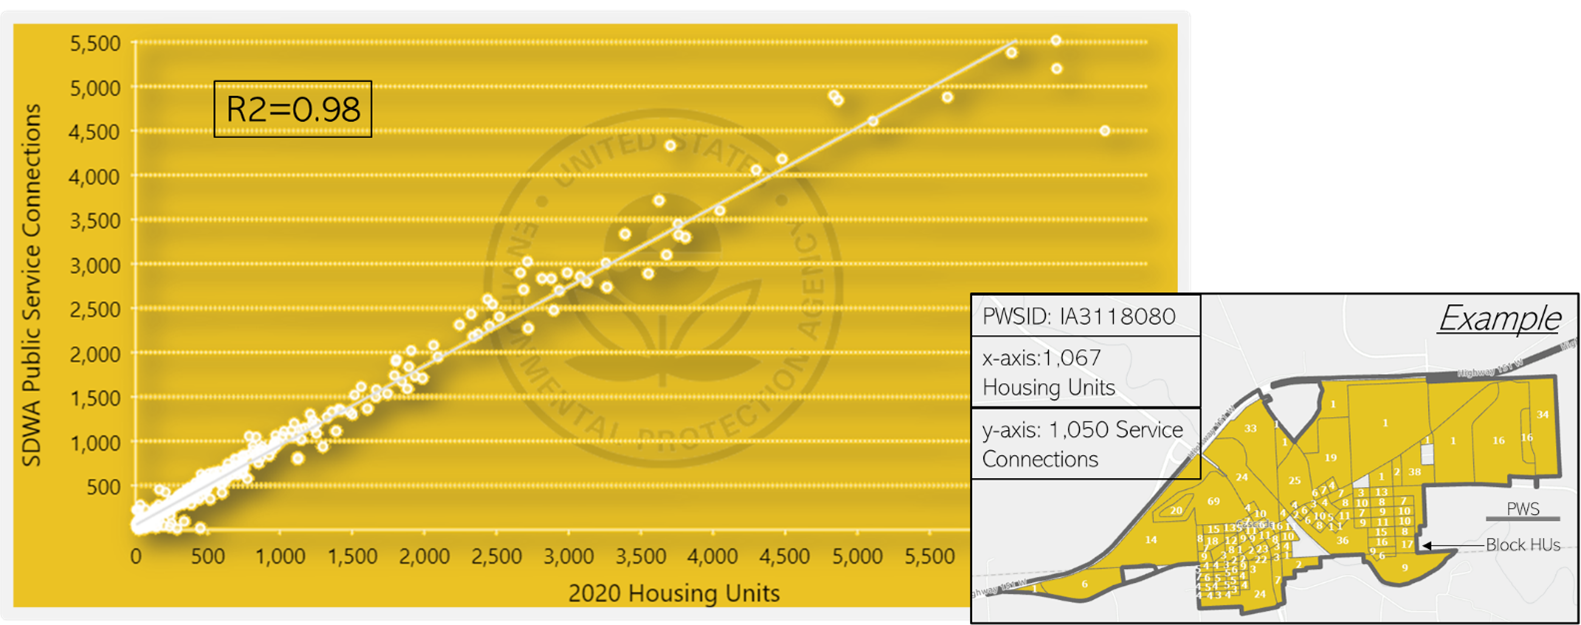
\includegraphics{img/IA_Regression.png}

}

\caption{\label{fig-IA}example of ``matched'' 1:1 systems using the
graphical regression method. These systems have a strong correlation
between housing units (x) and reported service connections (y). The
bottom right image shows how census block housing units are aggregated
per unique PWS}

\end{figure}%

\subsection{Random Forest}\label{random-forest}

The goal of the random forest model is to be able to determine what
public water system (or PWSID) a census block is most likely to be
served by. For example, a block in a rural area that is using public
water may be more likely to be close to its source water intake if it is
a very small system and more likely to be farther away if it a very
large rural water district. If you are served by a system that purchases
all of its water, the infrastructure may be farther away as well.

The random forest is set up to evaluate the relationship between a
single census block and a single point (facility location) associated
with a public water system. The tabular data used to train and apply the
random forest model has one row for the relationship between every block
and every unique PWSID within 25 miles (as determined by CWS
infrastructure such as wells, treatment plants, facility addresses, and
intakes). As an example, if there are seven different facilities within
twenty-five miles of a census block, the table used for the random
forest will have seven rows for that census block. Each facility is
associated with a parent PWSID. The random forest model then predicts a
probability that the parent PWSID is serving the census block in the
same row of the table. Predictor variables can be thought of as
belonging to one of two groups:

\begin{itemize}
\tightlist
\item
  Variables that that characterize the census block
\item
  Variables that characterize the water system.
\end{itemize}

The random forest model then determines the correct interplay between
the variables to determine a probability that a particular system serves
a particular census block or is not served by a public water system at
all.

\subsubsection{Variables that Describe the Census
Block}\label{variables-that-describe-the-census-block}

\paragraph{Population}\label{population}

Variable Name: \texttt{Population}

Population is taken from the 2020 Census, obtained at the census block
level from `2020\_DHCa' downloaded from NHGIS
(\citeproc{ref-manson2023ipums}{Manson et al. 2023}).

\paragraph{Local Population Density}\label{local-population-density}

Variable Name: \texttt{Pop\_km}

The centroid of each block is buffered by 2 miles (3,218.69 meters). The
population density is then calculated as an areal weighted population
density of census blocks that intersect the buffer. This variable
informs each block of its surroundings---in particular how dense is the
nearby city, suburb or rural area.

\paragraph{Area}\label{area}

Variable Name: \texttt{Area\_Km}

Area is calculated for each block in square kilometers using the Albers
equal area projection (crs = 5070).

\paragraph{Probability of Public
Water}\label{probability-of-public-water}

Variable Name: \texttt{Prob\_Pub}

The probability (0-1) of a block being served by public water as
estimated from the ORD water use decision tree model
(Figure~\ref{fig-dt}).

\paragraph{Buildings}\label{buildings}

Variable Name: \texttt{nBuildings}

The number of buildings within a census block that are greater then 50
square meters in area. This is calculated using Microsoft building
footprints (\citeproc{ref-mbfp}{Microsoft 2023}). We use a cutoff of 50
square meters to remove smaller buildings such as detached garages and
sheds (Figure~\ref{fig-mbfp}).

\begin{figure}

\centering{

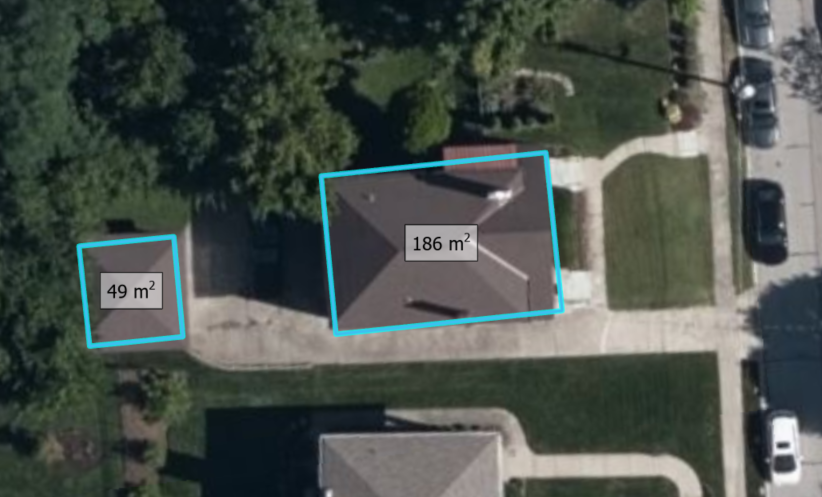
\includegraphics[width=4in,height=\textheight]{img/mbfp.png}

}

\caption{\label{fig-mbfp}Aerial image showing Microsoft building
footprints of a larger two-car garage and a residential home.
Annotations show the garage is just under fifty square meters.}

\end{figure}%

\paragraph{Percent Buildings}\label{percent-buildings}

Variable Name: \texttt{PctBldg}

The percent area of the census block that is covered by buildings. This
is calculated as the total area of microsoft building footprints divided
by the area of the census block (\citeproc{ref-mbfp}{Microsoft 2023}).

\paragraph{Mean Building Area}\label{mean-building-area}

Variable Name: \texttt{meanBldg\_m}

The mean area in square meters of buildings within the census block
(\citeproc{ref-mbfp}{Microsoft 2023}).

\paragraph{Minimum Building Area}\label{minimum-building-area}

Variable Name: \texttt{minBldg\_m}

The area in square meters of the smallest building within the census
block (Only buildings greater than or equal to 50 square meters
included) (\citeproc{ref-mbfp}{Microsoft 2023}).

\paragraph{Maximum Building Area}\label{maximum-building-area}

Variable Name: \texttt{maxBldg\_m}

The area in square meters of the largest building within the census
block (Only buildings greater than or equal to 50 square meters
included) (\citeproc{ref-mbfp}{Microsoft 2023}).

\paragraph{Standard Deviation of Building
Area}\label{standard-deviation-of-building-area}

Variable Name: \texttt{sdBldg\_m}

The standard deviation of area of buildings in square meters within a
census block (\citeproc{ref-mbfp}{Microsoft 2023}).

\paragraph{Rural / Urban}\label{rural-urban}

Variable Name: \texttt{PctRural}

The census defined urban / rural classifier; A binary classification, in
which to qualify as an urban area, the block identified must encompass
at least 2,000 housing units or have a population of at least 5,000 for
2020 (census block level). The dataset used is `Urban and Rural' from
`2020\_DHCa' at the census block level, obtained from NHGIS
(\citeproc{ref-manson2023ipums}{Manson et al. 2023})

\paragraph{Mean Residential Acres}\label{mean-residential-acres}

Variable Name: \texttt{meanResAcres}

The mean value in acres of parcels within the census block that are
zoned for residential use (\citeproc{ref-regrid}{REGRID 2023}).

\paragraph{Count of Parcels}\label{count-of-parcels}

Variable Name: \texttt{nParcels}

The total count of parcels within the census block
(\citeproc{ref-regrid}{REGRID 2023}).

\paragraph{Count of Mobile Homes}\label{count-of-mobile-homes}

Variable Name: \texttt{MH\_Count}

The count of mobile home communities within a census block as derived
from the Homeland Infrastructure Foundation Level database
(\citeproc{ref-hifld}{HIFLD 2023}).

\paragraph{Mobile Home Size}\label{mobile-home-size}

Variable Name: \texttt{MH\_Size}

The cumulative size of mobile home parks within a census block
representing the number of mobile home units (\citeproc{ref-hifld}{HIFLD
2023}). This variable is presented as a factor.

\textbf{Possible Values:}

\begin{longtable}[]{@{}ll@{}}
\toprule\noalign{}
Value & Description \\
\midrule\noalign{}
\endhead
\bottomrule\noalign{}
\endlastfoot
`50' & \textless50 Mobile Homes \\
`75' & 50-100 Mobile Homes \\
`100' & \textgreater100 Mobile Homes \\
\end{longtable}

\subsubsection{Variables that Describe the Closest
Systems}\label{variables-that-describe-the-closest-systems}

\paragraph{Distance}\label{distance}

Variable Name: \texttt{Facility\_Dist} The distance in meters between
the census block centroid and a single point from SDWIS for a system.

\paragraph{Distance Rank}\label{distance-rank}

Variable Name: \texttt{Dist\_Rank}

Describes the closeness rank of the particular facility being measured
to. For example, if \texttt{Dist\_Rank\ =\ 5}, there would be 4 other
facility points closer to the centroid of that census block.

\paragraph{Facility Type}\label{facility-type}

Variable Name: \texttt{Facility\_Type}

The type of system point that was used in the distance calculation.
Options include:

\begin{itemize}
\tightlist
\item
  ``Well''
\item
  ``Treatment Plant''
\item
  ``Consecutive Connection''
\item
  ``Intake''
\item
  ``Other''
\end{itemize}

The `Other' Category contains less frequent data and data used when
there are no wells, intakes or treatment plants associated with a
system. Some examples of less frequent locations are springs, reservoirs
and infiltration zones. This class also contains the administrative
contact addresses of systems as reported to SDWIS which are typically
within a service area but are also known to be unreliable depending on
the system. Administrative contact addresses were geolocated and curated
to only include street intersections or better.

\paragraph{Population Served}\label{population-served}

Variable Name: \texttt{Population\_Served\_Count}

The reported population that is served by the system in SDWIS reporting.

\paragraph{Connections}\label{connections}

Variable Name: \texttt{Service\_Connections\_Count}

The reported number of service connections within a system in SDWIS
reporting.

\paragraph{Distance to Center of
System}\label{distance-to-center-of-system}

Variable Name: \texttt{Ctr\_Dist}

If a system has more than one SDWIS point (intakes, wells treatment
plants etc\ldots) the mean center of all points is calculated and
measured in meters from the centroid of the census block. If only one
point exists within a system, this value will be identical to
\texttt{Facility\_Dist}.

\paragraph{System Type}\label{system-type}

Variable Name: \texttt{Service\_Area\_Type}

The Primary type of area that is served by the public water system.

\textbf{Possible Values:}

\begin{itemize}
\tightlist
\item
  `Homeowners Association'
\item
  `Mobile Home Park'
\item
  `Multiple'
\item
  `Municipality'
\item
  `Other'
\item
  `Residential Area'
\item
  `Subdivision'
\end{itemize}

\paragraph{Sub-County Match}\label{sub-county-match}

Variable Name: \texttt{SubCounty\_Match}

Reflects a classified Jaro-Winkler string distance between the census
place the census block is within and the `City Served' of the public
water system associated with the point being measured to.

\begin{longtable}[]{@{}ll@{}}
\toprule\noalign{}
Jaro-Winkler Distance & Classification \\
\midrule\noalign{}
\endhead
\bottomrule\noalign{}
\endlastfoot
\textless0.1 & ``Full Match'' \\
\textgreater0.1 \& \textless0.3 & ``Partial Match'' \\
≥0.3 & ``No Match'' \\
if no census sub county & ``No SubCounty'' \\
if no city served & ``No City Served'' \\
\end{longtable}

\paragraph{Place Match}\label{place-match}

Variable Name: \texttt{Place\_Match}

Reflects a classified Jaro-Winkler string distance between the census
place the census block is within and the `City Served' of the public
water system associated with the point being measured to.

\begin{longtable}[]{@{}ll@{}}
\toprule\noalign{}
Jaro-Winkler Distance & Classification \\
\midrule\noalign{}
\endhead
\bottomrule\noalign{}
\endlastfoot
\textless0.1 & ``Full Match'' \\
\textgreater0.1 \& \textless0.3 & ``Partial Match'' \\
≥0.3 & ``No Match'' \\
if no census place & ``No Place'' \\
if no city served & ``No City Served'' \\
\end{longtable}

\paragraph{County Match}\label{county-match}

Variable Name: \texttt{County\_Match}

A categorical value denoting whether the county that the census block is
within matches a county reported to be served by the system being
measured.

\textbf{Possible Values:}

\begin{itemize}
\tightlist
\item
  `Match'
\item
  `No Match'
\item
  `No County'
\end{itemize}

\paragraph{Place Name Present in System
Name}\label{place-name-present-in-system-name}

Variable Name: \texttt{Place\_in\_PWS}

A measure of how much of the system name also appears in the census
place name that the census block is within. The longest common
sub-string (LCS) is calculated between the census place and the system
name and is then using the formula:

\[(pwsName_{length}-LCS)/Place_{length}\] where \(pwsName_{length}\) is
the length of the place name string in characters, \(Place_{length}\) is
the length of the public water system name in characters and \(LCS\) is
the length of the longest common sub-string between the two. An exact
match would result in a value of 1. If either string is missing, a value
of zero is assigned.

\paragraph{Sub-County Name Present in System
Name}\label{sub-county-name-present-in-system-name}

Variable Name: \texttt{SC\_in\_PWS}

A measure of how much of the system name also appears in the census
sub-county name that the census block is within. The longest common
sub-string (LCS) is calculated between the census sub-county and the
system name and is then using the formula:

\[(pwsName_{length}-LCS)/SubCounty_{length}\] where \(pwsName_{length}\)
is the length of the sub-county name string in characters,
\(SubCounty_{length}\) is the length of the public water system name in
characters and \(LCS\) is the length of the longest common sub-string
between the two. An exact match would result in a value of 1. If either
string is missing, a value of zero is assigned.

\subsubsection{Training \& Validation}\label{training-validation}

The random forest is applied to every census block that is not covered
by an authoritative boundary (i.e.~state dataset) or captured by the 1:1
or mobile home methods, and returns a probability for each facility
location (excluding systems where authoritative and 1:1 boundaries
exist) within 25 miles of each census block. That probability can be
interpreted as the probability that the system PWSID associated with
that facility is serving public water to that census block. A full
comparison between the training and testing sets is shown in
Table~\ref{tbl-train}

The data used to build the random forest model was split randomly across
Arizona, Arkansas, California, Connecticut, New Jersey and Texas into
training and testing sets (Table~\ref{tbl-train}). These six states were
chosen due to their relative accuracy and completeness when inspected
and evaluated against the current universe of active community water
systems. Data is split into separate sets so the relationships
constructed by the random forest model can be evaluated against data it
has not been exposed to (out-of-bag sample).

\begin{longtable}[]{@{}lll@{}}
\caption{Summary statistics of the training and testing sets used to
build the random forest.}\label{tbl-train}\tabularnewline
\toprule\noalign{}
& Training Set & Testing Set \\
\midrule\noalign{}
\endfirsthead
\toprule\noalign{}
& Training Set & Testing Set \\
\midrule\noalign{}
\endhead
\bottomrule\noalign{}
\endlastfoot
\# Rows & 3.1 Million & 47 Million \\
\# Census Blocks & 760 Thousand & 1.1 Million \\
\# Correct & 350 Thousand & 4.2 Million \\
\# Incorrect & 2.8 Million & 42.7 Million \\
\# Systems & 1.7 Thousand & 1.7 Thousand \\
\end{longtable}

The random forest model was tuned on the number of trees and the value
of m-try (the number of random variables considered at each split). The
final model used a forest of fifty decision trees with \(m_{try}=20\).
The out-of-bag testing set returned 4,201,409 `TRUE' predictions (the
system PWSID is correct) and 42,738,447 `FALSE' predictions (the system
PWSID is not correct) and predicted 99.7\% of rows correctly. The
sensitivity (accuracy of true positives) was 98.38\% and the specificity
(accuracy of true negatives) was 99.83\%. The kappa value for the entire
testing set was 0.982.

The area under the curve (AUC) was calculated for the entire training
set, as well as subsets based on the number of service connections of
candidate systems for each census block (Figure~\ref{fig-rfAUC}). The
global auc for the testing set was 0.9997. The model AUC does decline as
systems become smaller. The AUC for systems with service connections
less than 500 was 0.9962.

\begin{figure}

\centering{

\includegraphics{Documentation_files/figure-pdf/fig-rfAUC-1.pdf}

}

\caption{\label{fig-rfAUC}Line and scatter plot showing that as service
connections increase, so does the AUC of the random forest model.}

\end{figure}%

\section{Post Processing}\label{post-processing}

The random forest model was post processed to simplify the boundary
results and remove spatial outliers.

\subsection{Hole Filling}\label{hole-filling}

Random forest outputs were spatially aggregated from the census block to
the PWSID. To overcome spatial issues, such as interstate highways and
right-of-ways, blocks were buffered by one-hundred meters, dissolved on
the PWSID, then negatively buffered by one-hundred meters to conserve
the correct footprint. A function to remove interior holes
(\citeproc{ref-nngeo}{Dorman 2022}).

\subsection{Polygon Part Removal
(Distance)}\label{polygon-part-removal-distance}

For random forest outputs, if a system had more than one polygon that
did not connect, we measured the distance between the largest polygon
for the system and each of the satellite polygons. If the satellite
polygon was more than ten kilometers away and had a lesser probability
than the primary polygon, it was deleted.

\subsection{Polygon Part Removal
(Area)}\label{polygon-part-removal-area}

It was discovered that there were many small ``artifacts'' the model
created: small in size and mostly isolated blocks that were relatively
far away from where their parent (primary---or largest) system boundary
was located. To carefully remove these, the features were `exploded' so
unique polygon parts could be examined individually. Before `explosion',
the total aggregate system size was calculated (Km2). The exploded
polygon parts size was then calculated (Km2), and each polygon part area
was divided by the total system area in order to get a percent of total
area. To remove these fragments, a threshold was applied: any polygon
part that was less than 20\% of the total system area and was less than
3 km2 in size was removed. This eliminated some 100k polygon parts.
After this procedure, only \textasciitilde48,000 polygon parts remained
(close to the number of total systems---suggesting most systems now only
have 1 polygon per system.

\section{Dataset Universe \& Known
Issues}\label{dataset-universe-known-issues}

The universe of systems we attempt to model is 47,952 systems. We were
able to model or gather state supplied boundaries for 42,743 systems
(89\%). The unmatched systems predominately serve relatively small
populations. This is proven when we calculate the percent of the
population served by modeled boundaries vs the universe of systems:
98.3\%. This high percentage gives us confidence that we are capturing
the service area boundaries for most people reliant on public water.
Figure 7 shows the percent of modeled/state supplied boundaries and
their percent population served of the total universe.

We remove any system that serves less than 25 people or has less than 15
service connections (unless we were able to model them or they were
state supplied)\footnote{This is similar to the EPA definition of a
  public water provider: ``A public water system provides water for
  human consumption through pipes or other constructed conveyances to at
  least 15 service connections or serves an average of at least 25
  people for at least 60 days a year.''
  https://www.epa.gov/dwreginfo/information-about-public-water-systems}.
These systems are typically sub-block in size and cannot reasonably be
modeled. A large majority of these systems also did not meet the federal
definition of a public water system.\\
Systems that are exclusively wholesalers of water were also removed from
the universe because these systems don't distribute water to
customers---and thus have no service area boundaries. Puerto Rico and US
territory systems are not included because explanatory data for model
inputs are not available for these geographies.

The final output dataset includes 44,415 systems out of a universe of
47,538 (93.4\%)

\subsection{Population Served by
State}\label{population-served-by-state}

The modeled boundaries represent 98.3 \% of the population served as
reported in SDWIS (Figure~\ref{fig-statePopServed}).

\begin{figure}

\centering{

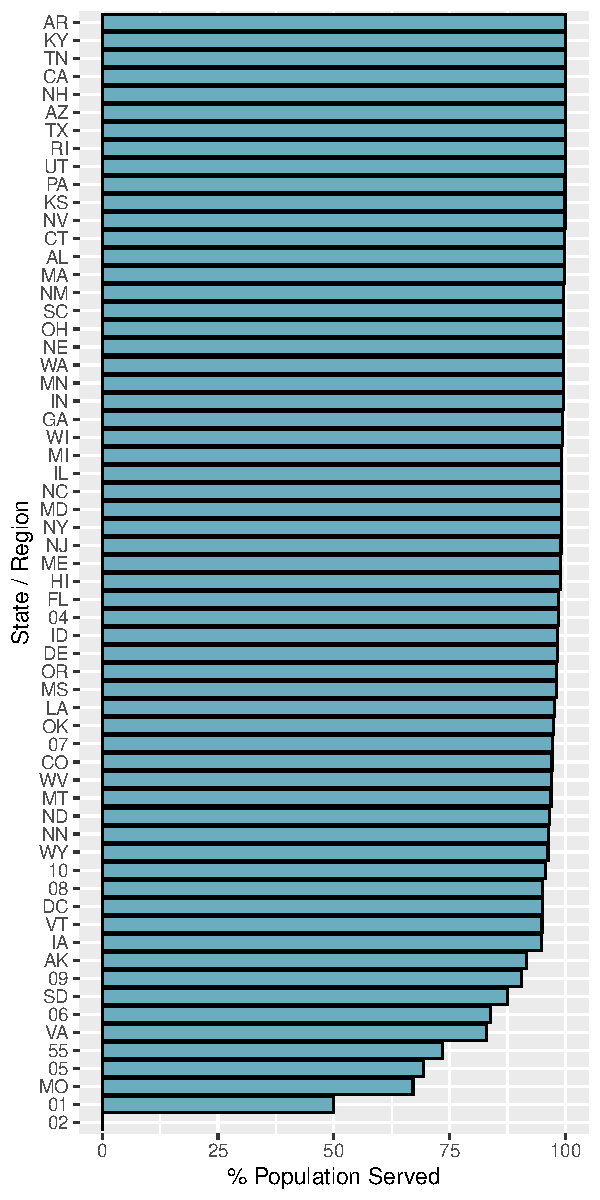
\includegraphics{Documentation_files/figure-pdf/fig-statePopServed-1.pdf}

}

\caption{\label{fig-statePopServed}Bar plot showing the percent of
population served by state or region that is captured by service area
boundaries. Regions refer to tribal systems within that EPA region.}

\end{figure}%

\subsection{Overlapping Boundaries}\label{overlapping-boundaries}

Within the final dataset there are instances where two or more
boundaries occupy the same area. Theoretically two or more systems can
occupy a single block (the spatial scale of the model) but this is known
to be rare. Overlaps usually occur in two scenarios:

\begin{enumerate}
\def\labelenumi{\arabic{enumi}.}
\tightlist
\item
  State boundaries overlapping modeled boundaries:
  Figure~\ref{fig-overlap1} shows an example of areas in Des Moines
  where boundaries overlap. Altoona, IA (modeled) overlaps the state
  supplied boundary of Des Moines. In this example the modeled boundary
  for Altoona appears correct. Altoona has a unique PWS. However, the
  state supplied boundary didn't ``erase'' the Altoona system from the
  service area. This conflict is likely a function of inaccurate state
  supplied boundaries.
\end{enumerate}

\begin{figure}

\centering{

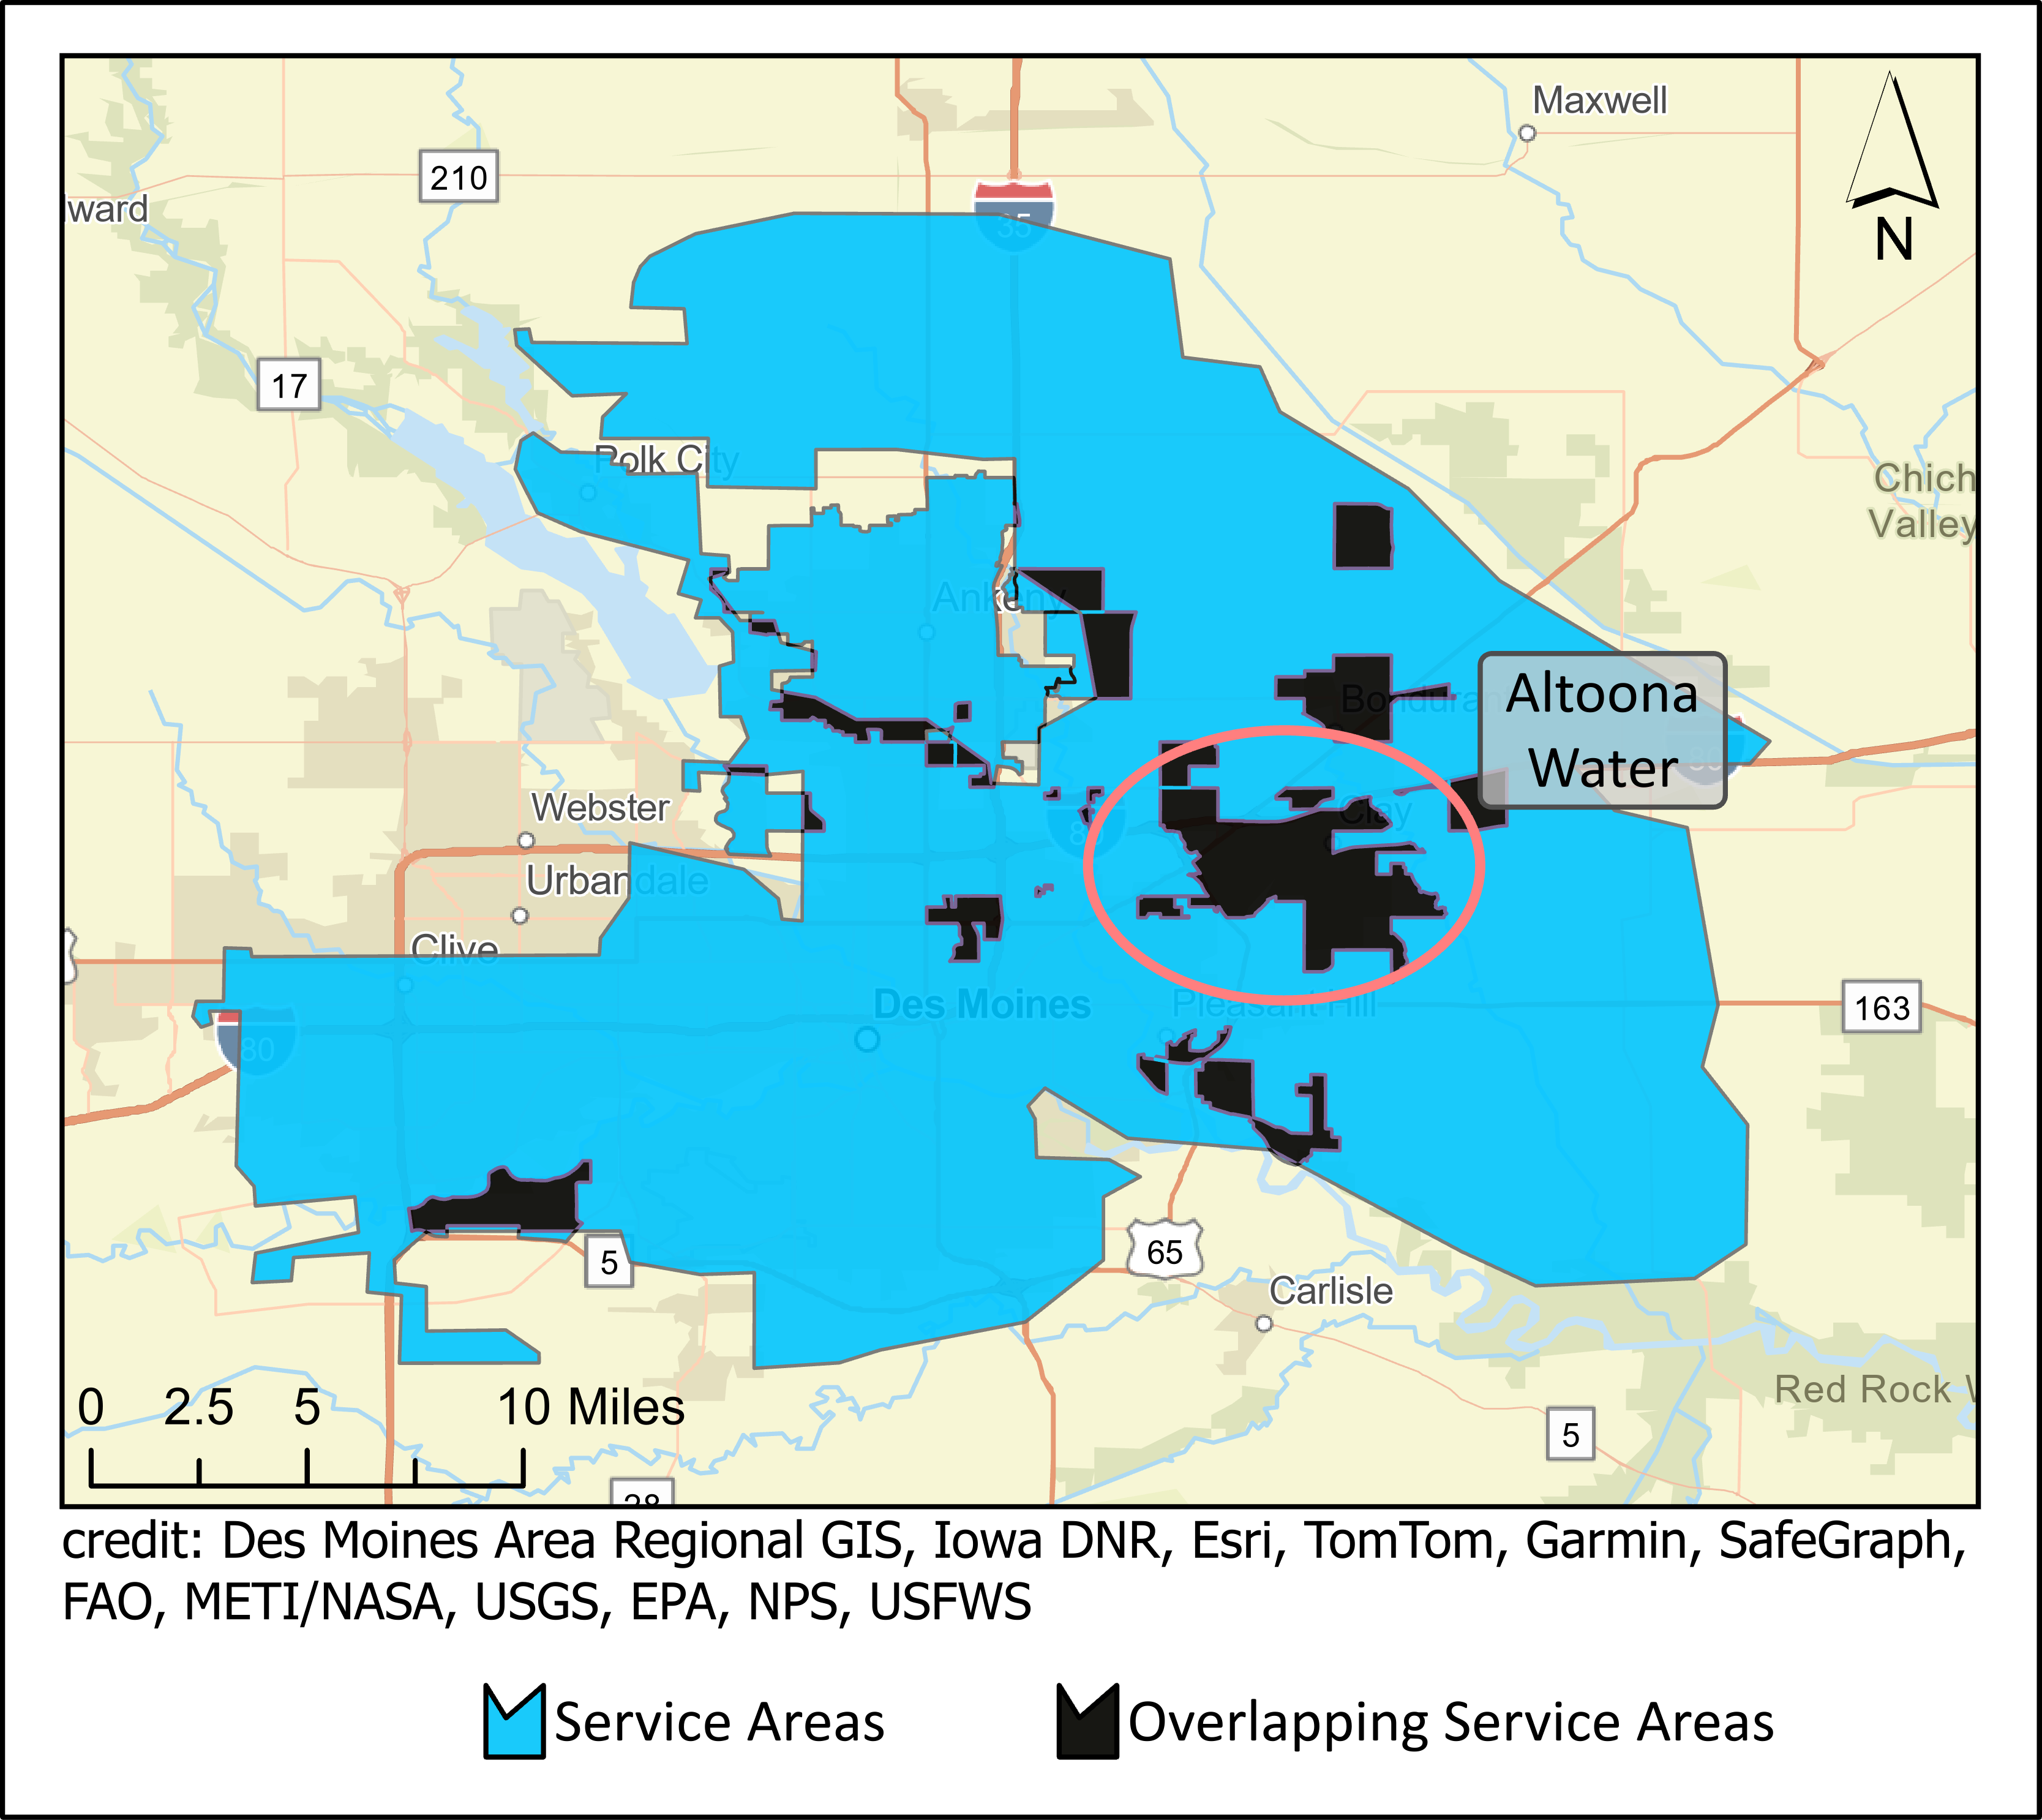
\includegraphics{img/overlap.png}

}

\caption{\label{fig-overlap1}State boundary (blue) overlapping modeled
boundaries (black)}

\end{figure}%

\begin{enumerate}
\def\labelenumi{\arabic{enumi}.}
\setcounter{enumi}{1}
\tightlist
\item
  State boundaries overlapping other state boundaries:
  Figure~\ref{fig-overlap2} shows an example of multiple state systems
  overlapping each other. Because these are state supplied boundaries,
  nothing can be done to resolve this issue. They are either incorrectly
  drawn or multiple systems serve approximately the same areas.
\end{enumerate}

\begin{figure}

\centering{

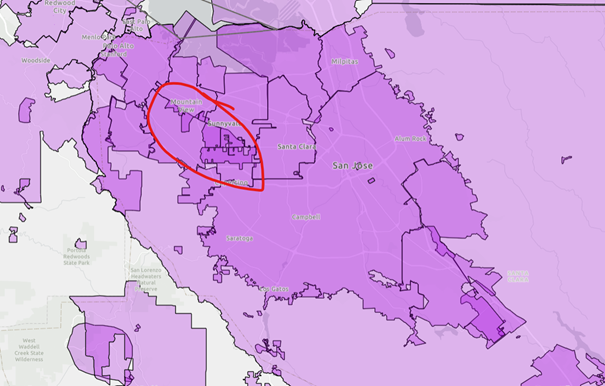
\includegraphics{img/overlap2.png}

}

\caption{\label{fig-overlap2}Map showing areas of overlap within state
supplied boundaries.}

\end{figure}%

\subsection{Incorrect Locations}\label{incorrect-locations}

All models have error. Trying to accurately model such a complex human
phenomenon such as public drinking water infrastructure is difficult.
The drivers that manifest a public drinking infrastructure---economic,
social, environmental---is also complex and varies from state-to-state,
community-to-community. The decision tree model was trained on 3 states
and the random forest was trained on 6 states. This limited geographic
range creates bias in the model and may not represent different drinking
water infrastructure assumptions that may be relevant in one state, but
not in others. One known issue is the poor accuracy of rural water
systems serving very rural geographies. Our decision tree dataset was
trained on states with a fairly urban population and states that didn't
have very many rural water districts to train the model on. South
Dakota, for example, is a state with many rural water districts that
cover large swaths of the rural landscape. We deliberately avoided
including such districts in our training dataset because rural water
districts are unique to only some states. Generally speaking, rural
farmland does not have public water---so we did not want to train a
model that saw farmland as being served by public water. Because of this
model bias, modeled rural water districts are a known issue in our model
and are typically not modeled accurately.

\subsection{Missing Systems}\label{missing-systems}

Why can some systems not be modeled? Besides the issue of systems being
too small to model, there is another reason. The model requires
geographic signals, or clues, to accurately place a service area
boundary on the map. These geographic clues come primarily from two
sources: 1.) SDWIS locations such as wells, intakes, and treatment
plants and 2.) SDWIS reported system information such as `City Served'.
These signals help the model triangulate an appropriate geography for
the service area. Approximately a dozen states don't report ``City
Served'. In addition some systems don't have corresponding SDWIS point
locations or the information they provide is incorrect. For these
reasons, a good portion of the systems that could not be modeled were
not modeled. For example, Figure~\ref{fig-missingCon} shows the vast
majority of systems we could not model report less than 100 connections.
Certain types of systems are also difficult to model. As represented in
Figure~\ref{fig-missingType}, the areas we struggle to model are areas
like mobile home park or subdivisions.

\begin{figure}

\centering{

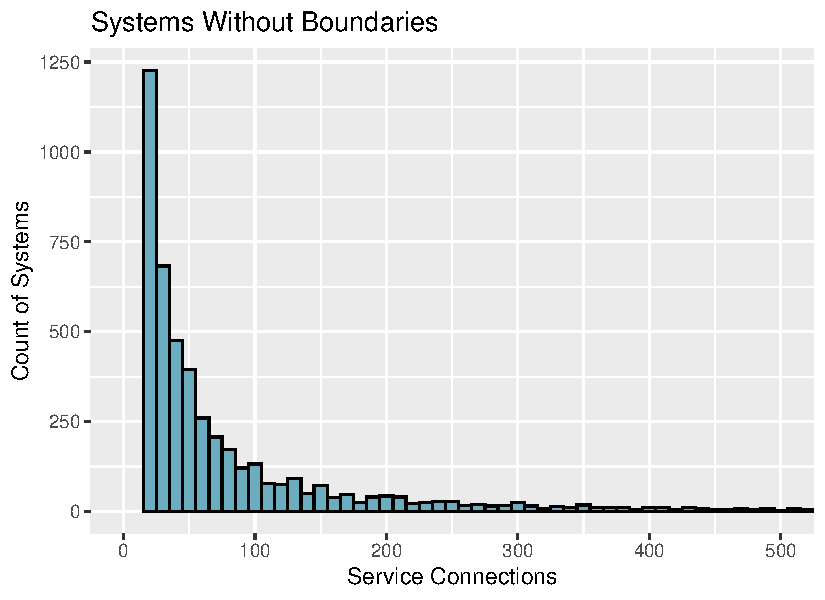
\includegraphics{Documentation_files/figure-pdf/fig-missingCon-1.pdf}

}

\caption{\label{fig-missingCon}Histogram of systems we do not have
boundaries for by the number of service connections reported under SDWA.
binwidth = 10 connections.}

\end{figure}%

\begin{figure}

\centering{

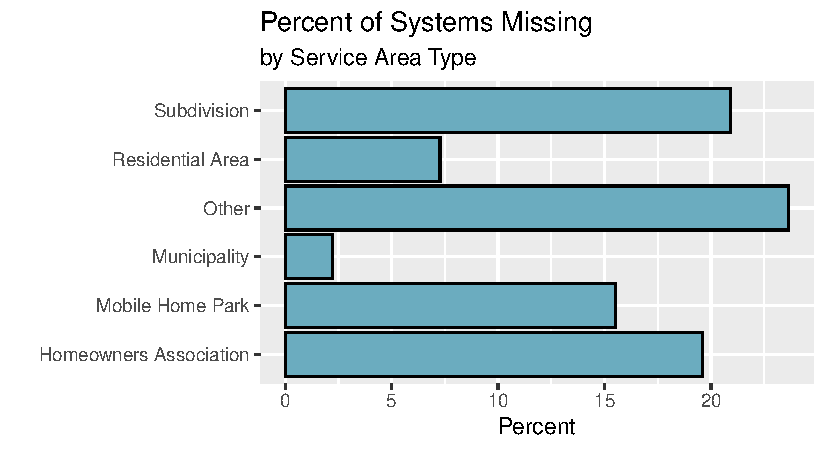
\includegraphics{Documentation_files/figure-pdf/fig-missingType-1.pdf}

}

\caption{\label{fig-missingType}Bar plot showing the percent of systems
missing boundaries by the type of area they primarily serve.}

\end{figure}%

\subsection{Kentucky}\label{kentucky}

According to the state of Kentucky, about 95\% of Kentuckians have
access to public drinking water (\citeproc{ref-kydow}{Water 2022}).
Kentucky is relatively unique in the broad reach of their water systems
to rural areas. While Kentucky does not publish service area boundaries.
We received water line data from the state of kentucky, associated with
PWSIDs, which delineated the main water lines. To delineate service
areas, Voronoi polygons (also known as Thiessen polygons) were generated
from service line data. It should be noted that the Voronoi polygons
were derived from state supplied data, but the polygons themselves are
not state supplied.

\subsection{Florida}\label{florida}

For some state supplied boundaries in Florida, one polygon was
associated with multiple PWSIDs. We are unable to disaggregate these
multiple systems from their single geography. For these features in the
dataset, you will see multiple PWSIDs within the `PWSID' field.

\section{Code and Additional
Resources}\label{code-and-additional-resources}

The data curation, modeling and analysis for this work was done using R
(\citeproc{ref-R}{R Core Team 2022}) and R Studio
(\citeproc{ref-rstudio}{Posit team 2023}). All code can be viewed in the
EPA agency GitHub page available at:
\url{https://github.com/USEPA/ORD_SAB_Model}. Additional information is
also available in this repository such as source information for
boundary data obtained from state and utility sources.

To view or download the data, visit the
\href{https://epa.maps.arcgis.com/apps/webappviewer/index.html?id=5a9963ca7a594fbd9b0df40050ed704e}{Service
Area web application}.

\section{Appendix}\label{appendix}

\subsection{Table of systems by Primacy Agency and
Method}\label{table-of-systems-by-primacy-agency-and-method}

\begin{longtable*}{rrrrrr}
\toprule
Random Forest & Decision Tree & OSM & Parcel & State & Census Place \\ 
\midrule\addlinespace[2.5pt]
\multicolumn{6}{l}{EPA Region 1} \\ 
\midrule\addlinespace[2.5pt]
1 & 0 & 0 & 0 & 0 & 0 \\ 
\midrule\addlinespace[2.5pt]
\multicolumn{6}{l}{EPA Region 10} \\ 
\midrule\addlinespace[2.5pt]
60 & 11 & 0 & 0 & 0 & 0 \\ 
\midrule\addlinespace[2.5pt]
\multicolumn{6}{l}{EPA Region 4} \\ 
\midrule\addlinespace[2.5pt]
12 & 0 & 0 & 0 & 0 & 0 \\ 
\midrule\addlinespace[2.5pt]
\multicolumn{6}{l}{EPA Region 5} \\ 
\midrule\addlinespace[2.5pt]
43 & 14 & 0 & 0 & 0 & 0 \\ 
\midrule\addlinespace[2.5pt]
\multicolumn{6}{l}{EPA Region 6} \\ 
\midrule\addlinespace[2.5pt]
38 & 3 & 0 & 0 & 0 & 0 \\ 
\midrule\addlinespace[2.5pt]
\multicolumn{6}{l}{EPA Region 7} \\ 
\midrule\addlinespace[2.5pt]
7 & 1 & 0 & 0 & 0 & 0 \\ 
\midrule\addlinespace[2.5pt]
\multicolumn{6}{l}{EPA Region 8} \\ 
\midrule\addlinespace[2.5pt]
70 & 21 & 0 & 0 & 0 & 0 \\ 
\midrule\addlinespace[2.5pt]
\multicolumn{6}{l}{EPA Region 9} \\ 
\midrule\addlinespace[2.5pt]
143 & 9 & 0 & 0 & 0 & 0 \\ 
\midrule\addlinespace[2.5pt]
\multicolumn{6}{l}{AK} \\ 
\midrule\addlinespace[2.5pt]
121 & 145 & 2 & 13 & 0 & 0 \\ 
\midrule\addlinespace[2.5pt]
\multicolumn{6}{l}{AL} \\ 
\midrule\addlinespace[2.5pt]
409 & 77 & 1 & 0 & 2 & 0 \\ 
\midrule\addlinespace[2.5pt]
\multicolumn{6}{l}{AR} \\ 
\midrule\addlinespace[2.5pt]
3 & 0 & 0 & 0 & 670 & 0 \\ 
\midrule\addlinespace[2.5pt]
\multicolumn{6}{l}{AZ} \\ 
\midrule\addlinespace[2.5pt]
25 & 0 & 1 & 3 & 707 & 0 \\ 
\midrule\addlinespace[2.5pt]
\multicolumn{6}{l}{CA} \\ 
\midrule\addlinespace[2.5pt]
25 & 0 & 0 & 0 & 2812 & 0 \\ 
\midrule\addlinespace[2.5pt]
\multicolumn{6}{l}{CO} \\ 
\midrule\addlinespace[2.5pt]
670 & 28 & 13 & 14 & 3 & 0 \\ 
\midrule\addlinespace[2.5pt]
\multicolumn{6}{l}{CT} \\ 
\midrule\addlinespace[2.5pt]
22 & 2 & 0 & 0 & 448 & 0 \\ 
\midrule\addlinespace[2.5pt]
\multicolumn{6}{l}{DC} \\ 
\midrule\addlinespace[2.5pt]
1 & 0 & 0 & 0 & 1 & 0 \\ 
\midrule\addlinespace[2.5pt]
\multicolumn{6}{l}{DE} \\ 
\midrule\addlinespace[2.5pt]
146 & 12 & 9 & 11 & 0 & 0 \\ 
\midrule\addlinespace[2.5pt]
\multicolumn{6}{l}{FL} \\ 
\midrule\addlinespace[2.5pt]
860 & 56 & 13 & 1 & 464 & 0 \\ 
\midrule\addlinespace[2.5pt]
\multicolumn{6}{l}{GA} \\ 
\midrule\addlinespace[2.5pt]
1283 & 91 & 6 & 24 & 3 & 0 \\ 
\midrule\addlinespace[2.5pt]
\multicolumn{6}{l}{HI} \\ 
\midrule\addlinespace[2.5pt]
83 & 15 & 0 & 0 & 0 & 0 \\ 
\midrule\addlinespace[2.5pt]
\multicolumn{6}{l}{IA} \\ 
\midrule\addlinespace[2.5pt]
855 & 114 & 11 & 8 & 2 & 0 \\ 
\midrule\addlinespace[2.5pt]
\multicolumn{6}{l}{ID} \\ 
\midrule\addlinespace[2.5pt]
544 & 27 & 15 & 5 & 2 & 0 \\ 
\midrule\addlinespace[2.5pt]
\multicolumn{6}{l}{IL} \\ 
\midrule\addlinespace[2.5pt]
1445 & 138 & 34 & 17 & 0 & 0 \\ 
\midrule\addlinespace[2.5pt]
\multicolumn{6}{l}{IN} \\ 
\midrule\addlinespace[2.5pt]
499 & 116 & 25 & 105 & 2 & 0 \\ 
\midrule\addlinespace[2.5pt]
\multicolumn{6}{l}{KS} \\ 
\midrule\addlinespace[2.5pt]
61 & 5 & 4 & 3 & 781 & 0 \\ 
\midrule\addlinespace[2.5pt]
\multicolumn{6}{l}{KY} \\ 
\midrule\addlinespace[2.5pt]
7 & 0 & 0 & 0 & 370 & 0 \\ 
\midrule\addlinespace[2.5pt]
\multicolumn{6}{l}{LA} \\ 
\midrule\addlinespace[2.5pt]
779 & 31 & 0 & 8 & 1 & 0 \\ 
\midrule\addlinespace[2.5pt]
\multicolumn{6}{l}{MA} \\ 
\midrule\addlinespace[2.5pt]
437 & 6 & 0 & 15 & 2 & 0 \\ 
\midrule\addlinespace[2.5pt]
\multicolumn{6}{l}{MD} \\ 
\midrule\addlinespace[2.5pt]
324 & 25 & 10 & 19 & 0 & 0 \\ 
\midrule\addlinespace[2.5pt]
\multicolumn{6}{l}{ME} \\ 
\midrule\addlinespace[2.5pt]
266 & 21 & 2 & 7 & 0 & 0 \\ 
\midrule\addlinespace[2.5pt]
\multicolumn{6}{l}{MI} \\ 
\midrule\addlinespace[2.5pt]
1052 & 120 & 9 & 43 & 2 & 0 \\ 
\midrule\addlinespace[2.5pt]
\multicolumn{6}{l}{MN} \\ 
\midrule\addlinespace[2.5pt]
789 & 83 & 8 & 28 & 0 & 0 \\ 
\midrule\addlinespace[2.5pt]
\multicolumn{6}{l}{MO} \\ 
\midrule\addlinespace[2.5pt]
1196 & 73 & 3 & 0 & 0 & 1 \\ 
\midrule\addlinespace[2.5pt]
\multicolumn{6}{l}{MS} \\ 
\midrule\addlinespace[2.5pt]
585 & 36 & 0 & 0 & 361 & 0 \\ 
\midrule\addlinespace[2.5pt]
\multicolumn{6}{l}{MT} \\ 
\midrule\addlinespace[2.5pt]
471 & 29 & 7 & 89 & 1 & 0 \\ 
\midrule\addlinespace[2.5pt]
\multicolumn{6}{l}{NC} \\ 
\midrule\addlinespace[2.5pt]
1084 & 20 & 7 & 145 & 483 & 0 \\ 
\midrule\addlinespace[2.5pt]
\multicolumn{6}{l}{ND} \\ 
\midrule\addlinespace[2.5pt]
247 & 39 & 0 & 0 & 0 & 0 \\ 
\midrule\addlinespace[2.5pt]
\multicolumn{6}{l}{NE} \\ 
\midrule\addlinespace[2.5pt]
496 & 62 & 5 & 1 & 0 & 0 \\ 
\midrule\addlinespace[2.5pt]
\multicolumn{6}{l}{NH} \\ 
\midrule\addlinespace[2.5pt]
40 & 0 & 0 & 2 & 658 & 0 \\ 
\midrule\addlinespace[2.5pt]
\multicolumn{6}{l}{NJ} \\ 
\midrule\addlinespace[2.5pt]
4 & 1 & 0 & 0 & 560 & 0 \\ 
\midrule\addlinespace[2.5pt]
\multicolumn{6}{l}{NM} \\ 
\midrule\addlinespace[2.5pt]
26 & 1 & 0 & 0 & 532 & 0 \\ 
\midrule\addlinespace[2.5pt]
\multicolumn{6}{l}{NN} \\ 
\midrule\addlinespace[2.5pt]
114 & 8 & 0 & 0 & 4 & 0 \\ 
\midrule\addlinespace[2.5pt]
\multicolumn{6}{l}{NV} \\ 
\midrule\addlinespace[2.5pt]
132 & 20 & 2 & 5 & 1 & 0 \\ 
\midrule\addlinespace[2.5pt]
\multicolumn{6}{l}{NY} \\ 
\midrule\addlinespace[2.5pt]
1079 & 96 & 2 & 338 & 308 & 0 \\ 
\midrule\addlinespace[2.5pt]
\multicolumn{6}{l}{OH} \\ 
\midrule\addlinespace[2.5pt]
847 & 104 & 39 & 99 & 1 & 0 \\ 
\midrule\addlinespace[2.5pt]
\multicolumn{6}{l}{OK} \\ 
\midrule\addlinespace[2.5pt]
748 & 47 & 1 & 0 & 0 & 0 \\ 
\midrule\addlinespace[2.5pt]
\multicolumn{6}{l}{OR} \\ 
\midrule\addlinespace[2.5pt]
601 & 26 & 27 & 99 & 0 & 0 \\ 
\midrule\addlinespace[2.5pt]
\multicolumn{6}{l}{PA} \\ 
\midrule\addlinespace[2.5pt]
86 & 12 & 3 & 0 & 1770 & 0 \\ 
\midrule\addlinespace[2.5pt]
\multicolumn{6}{l}{RI} \\ 
\midrule\addlinespace[2.5pt]
40 & 1 & 0 & 9 & 31 & 0 \\ 
\midrule\addlinespace[2.5pt]
\multicolumn{6}{l}{SC} \\ 
\midrule\addlinespace[2.5pt]
419 & 51 & 3 & 31 & 2 & 0 \\ 
\midrule\addlinespace[2.5pt]
\multicolumn{6}{l}{SD} \\ 
\midrule\addlinespace[2.5pt]
355 & 35 & 2 & 3 & 0 & 0 \\ 
\midrule\addlinespace[2.5pt]
\multicolumn{6}{l}{TN} \\ 
\midrule\addlinespace[2.5pt]
16 & 1 & 0 & 0 & 445 & 0 \\ 
\midrule\addlinespace[2.5pt]
\multicolumn{6}{l}{TX} \\ 
\midrule\addlinespace[2.5pt]
71 & 2 & 0 & 0 & 4538 & 0 \\ 
\midrule\addlinespace[2.5pt]
\multicolumn{6}{l}{UT} \\ 
\midrule\addlinespace[2.5pt]
8 & 0 & 0 & 0 & 485 & 0 \\ 
\midrule\addlinespace[2.5pt]
\multicolumn{6}{l}{VA} \\ 
\midrule\addlinespace[2.5pt]
799 & 43 & 4 & 22 & 0 & 0 \\ 
\midrule\addlinespace[2.5pt]
\multicolumn{6}{l}{VT} \\ 
\midrule\addlinespace[2.5pt]
283 & 21 & 4 & 23 & 0 & 0 \\ 
\midrule\addlinespace[2.5pt]
\multicolumn{6}{l}{WA} \\ 
\midrule\addlinespace[2.5pt]
380 & 7 & 0 & 0 & 1747 & 0 \\ 
\midrule\addlinespace[2.5pt]
\multicolumn{6}{l}{WI} \\ 
\midrule\addlinespace[2.5pt]
768 & 107 & 21 & 12 & 2 & 0 \\ 
\midrule\addlinespace[2.5pt]
\multicolumn{6}{l}{WV} \\ 
\midrule\addlinespace[2.5pt]
139 & 9 & 0 & 11 & 253 & 1 \\ 
\midrule\addlinespace[2.5pt]
\multicolumn{6}{l}{WY} \\ 
\midrule\addlinespace[2.5pt]
226 & 17 & 4 & 2 & 0 & 0 \\ 
\midrule\addlinespace[2.5pt]
\multicolumn{6}{l}{NA} \\ 
\midrule\addlinespace[2.5pt]
21 & 0 & 0 & 0 & 45 & 0 \\ 
\bottomrule
\end{longtable*}

\phantomsection\label{refs}
\begin{CSLReferences}{1}{0}
\bibitem[\citeproctext]{ref-act1974safe}
Act, Safe Drinking Water. 1974. {``Safe Drinking Water Act.''} In
\emph{Enacted by the 93rd United States Congress. Effective}. Vol. 88.

\bibitem[\citeproctext]{ref-nngeo}
Dorman, Michael. 2022. \emph{Nngeo: K-Nearest Neighbor Join for Spatial
Data}. \url{https://CRAN.R-project.org/package=nngeo}.

\bibitem[\citeproctext]{ref-epaCompliance}
EPA, U. S. 2023. {``Providing Safe Drinking Water in America: National
Public Water Systems Compliance Report.''}
\url{https://www.epa.gov/compliance/providing-safe-drinking-water-america-national-public-water-systems-compliance-report}.

\bibitem[\citeproctext]{ref-cws}
EPA, US. 2022. {``Information about Public Water Systems.''}
\url{https://www.epa.gov/dwreginfo/information-about-public-water-systems}.

\bibitem[\citeproctext]{ref-hifld}
HIFLD. 2023. {``Homeland Infrastructure Foundation-Level Data.''}
\url{https://services1.arcgis.com/Hp6G80Pky0om7QvQ/arcgis/rest/services/Mobile_Home_Parks/FeatureServer/0}.

\bibitem[\citeproctext]{ref-manson2023ipums}
Manson, Steven M, Jonathan Schroeder, David Van Riper, Katherine
Knowles, Tracy Kugler, Finn Roberts, and Steven Ruggles. 2023. {``IPUMS
National Historical Geographic Information System: Version 18.0.''}

\bibitem[\citeproctext]{ref-mbfp}
Microsoft. 2023. {``US Building Footprints.''}
\url{https://github.com/microsoft/USBuildingFootprints?tab=readme-ov-file}.

\bibitem[\citeproctext]{ref-murray2021methods}
Murray, Andrew, Alexander Hall, James Weaver, and Fran Kremer. 2021.
{``Methods for Estimating Locations of Housing Units Served by Private
Domestic Wells in the United States Applied to 2010.''} \emph{JAWRA}.

\bibitem[\citeproctext]{ref-rstudio}
Posit team. 2023. \emph{RStudio: Integrated Development Environment for
r}. Boston, MA: Posit Software, PBC. \url{http://www.posit.co/}.

\bibitem[\citeproctext]{ref-R}
R Core Team. 2022. \emph{R: A Language and Environment for Statistical
Computing}. Vienna, Austria: R Foundation for Statistical Computing.
\url{https://www.R-project.org/}.

\bibitem[\citeproctext]{ref-regrid}
REGRID. 2023. {``REGRID Parcels Feature Service.''}
\url{https://epa.maps.arcgis.com/home/item.html?id=75da303642e74f4b8b25caa6c1bbfad0}.

\bibitem[\citeproctext]{ref-toccalino2010quality}
Toccalino, Patricia L, Julia E Norman, and Kerie J Hitt. 2010.
{``Quality of Source Water from Public-Supply Wells in the United
States, 1993-2007.''} US Geological Survey.

\bibitem[\citeproctext]{ref-kydow}
Water, Kentucky Division of. 2022. {``Drinking Water.''}
\url{https://eec.ky.gov/Environmental-Protection/Water/Drinking/Pages/Drinking\%20Water.aspx}.

\end{CSLReferences}

\end{document}
